% Copyright 2009--2010  Ed Bueler

%\documentclass[10pt,hyperref={pdfpagelabels=false}]{beamer}
\documentclass[10pt]{beamer}

\mode<presentation>
{
  \usetheme{Hannover}
  % or ...

  \usecolortheme{crane}

  \setbeamercovered{transparent}
  % or whatever (possibly just delete it)
  
  \setbeamerfont{frametitle}{size=\large}
}

\usepackage[english]{babel}
\usepackage[latin1]{inputenc}
\usepackage{times}
\usepackage[T1]{fontenc}
% Or whatever. Note that the encoding and the font should match. If T1
% does not look nice, try deleting the line with the fontenc.

\usepackage{empheq}
\usepackage{amsmath}
\usepackage{esint}
\usepackage{animate}
\usepackage{xspace}
\usepackage{verbatim}
\usepackage{hyperref}

% we can generate a reference list if bibtex is applied to this .tex,
%   and here's the style:
\usepackage{natbib}


\title[Numerical modelling]{
Numerical modelling \\ 
of ice sheets and ice shelves}

\author{Ed Bueler}

\institute{
Dept of Mathematics and Statistics \\
and Geophysical Institute \\
University of Alaska, Fairbanks}

\lecture[1]{Numerical modelling of ice sheets and ice shelves}{lecture-text}


\date{September 2010 \\ Karthaus Summer School}


% remove this when printing out:
\AtBeginSection[]
{
  \begin{frame}<beamer>
    \frametitle{Outline}
    \tableofcontents[currentsection,hideallsubsections]
  \end{frame}
}


% If you wish to uncover everything in a step-wise fashion, uncomment:
%\beamerdefaultoverlayspecification{<+->}

\newcommand{\bg}{\mathbf{g}}
\newcommand{\bq}{\mathbf{q}}
\newcommand{\bu}{\mathbf{u}}
\newcommand{\bw}{\mathbf{w}}

\newcommand{\bA}{\mathbf{A}}
\newcommand{\bbF}{\mathbf{F}}
\newcommand{\bU}{\mathbf{U}}

\newcommand{\ddt}[1]{\ensuremath{\frac{\partial #1}{\partial t}}}
\newcommand{\ddx}[1]{\ensuremath{\frac{\partial #1}{\partial x}}}
\newcommand{\ddy}[1]{\ensuremath{\frac{\partial #1}{\partial y}}}
\newcommand{\pp}[2]{\ensuremath{\frac{\partial #1}{\partial #2}}}
\renewcommand{\t}[1]{\texttt{#1}}
\newcommand{\eps}{\epsilon}
\newcommand{\grad}{\nabla}
\newcommand{\Div}{\nabla\cdot}
\newcommand{\strainrate}{D}
\newcommand{\devstress}{\tau}

\newcommand{\Matlab}{\textsc{Matlab}\xspace}
\newcommand{\Octave}{\textsc{Octave}\xspace}

\newcommand{\exer}[2]{\medskip\noindent \textbf{#1.}\quad #2}
\mode<presentation>{
\newcommand{\slidepage}[1]{slide \pageref{#1}}
}

\newcommand{\mname}[1]{\href{http://www.dms.uaf.edu/~bueler/karthaus/mfiles/#1}{\texttt{#1}}}

\newcommand{\txtinput}[1]{ \scriptsize \verbatiminput{#1} }

\newcommand{\txtinputtiny}[1]{ \tiny \verbatiminput{#1} }

\newcommand{\mmessage}[1]{\begin{center}
\emph{see code} \url{http://www.dms.uaf.edu/~bueler/karthaus/mfiles/#1.m}
\end{center}}

\newcommand{\mmess}[1]{\vspace{-0.1in}\begin{center}
\fbox{\url{http://www.dms.uaf.edu/~bueler/karthaus/mfiles/#1.m}}
\end{center}}


\newcommand{\minput}[1]{
\scriptsize \verbatiminput{mfiles/#1.slim.m}
\vspace{-0.2in}
\tiny \mmess{#1}
\normalsize
}


\newcommand{\minputtiny}[1]{
\tiny \verbatiminput{mfiles/#1.slim.m}
\vspace{-0.16in}
\mmess{#1}
\normalsize
}


\begin{document}

\begin{frame}
  \maketitle
\end{frame}

% the major parts are in separate files:


\section{introduction}

\begin{frame}{slogans \& scope}

slogans:
  \begin{enumerate}
  \item \alert{focus on approximating ice flow}
  \item \alert{example numerical codes that actually work}
  \end{enumerate}
\medskip

scope:
  \begin{itemize}
  \item[$\circ$] continuum models

    \begin{itemize}
    \item shallow ice approximation (SIA) in 2D
    \item shallow shelf approximation (SSA) in 1D
    \item mass continuity \& surface kinematical equations
    \end{itemize}

  \item[$\circ$] numerical ideas

    \begin{itemize}
    \item finite difference schemes
    \item solving algebraic systems from stress balances
    \item verification
    \end{itemize}
  \end{itemize}
\end{frame}


\begin{frame}{outside of scope}

\large\emph{not} \normalsize covered here:\normalsize
\medskip

  \begin{itemize}
  \item Stokes and ``higher order'' flow equations
  \item thermomechanical coupling or polythermal ice
  \item subglacial hydrology/processes
  \item mass balance and snow/firn processes
  \item constitutive relations other than Glen isotropic
  \item grounding lines, calving fronts, ocean interaction
  \item paleo-climate and ``spin-up''
  \item earth deformation under ice sheet load
  \item other numerics: FEM, spectral, multigrid, parallel, \dots
  \item etc.
  \end{itemize}

\end{frame}


\begin{frame}{notation} 

\begin{center}
  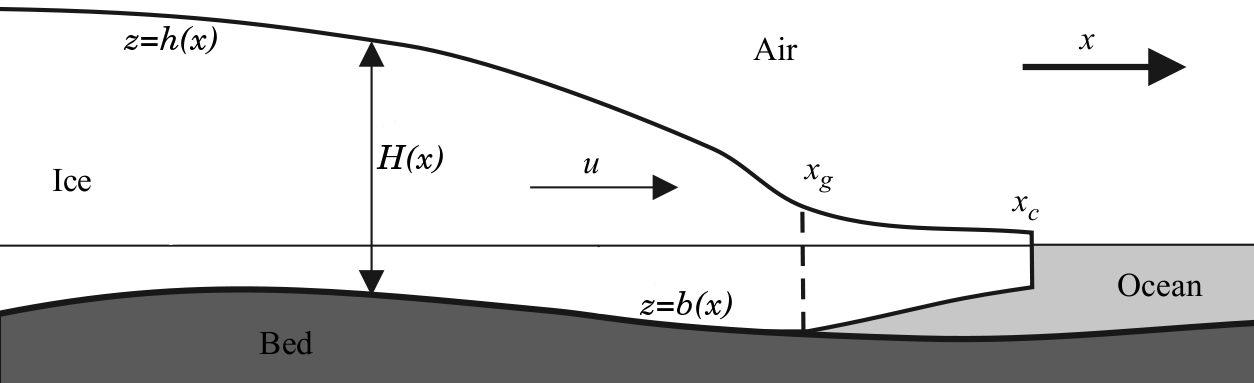
\includegraphics[width=0.9\textwidth]{flowline}

\tiny \emph{figure modified from} Schoof (2007)\nocite{SchoofMarine1}
\end{center}

\scriptsize
  \begin{itemize}
  \item coordinates $t,x,y,z$  (with $z$ vertical, positive upward)
  \item subscripts for partial derivatives $u_x = \partial u/\partial x$
  \item $H=$ ice thickness
  \item $h=$ ice surface elevation
  \item $b=$ bedrock surface elevation
  \item $T=$ ice temperature
  \item $\mathbf{u}=(u,v,w)=$ ice velocity
  \item $\rho=$ density of ice
  \item $\rho_w=$ density of ocean water
  \item $g=$ acceleration of gravity
  \item $n=3$ Glen flow law exponent $=3$
  \item $A=A(T)=$ ice softness in Glen law ($\mathbf{D}_{ij} = A(T) \tau^{n-1} \tau_{ij}$)
  \item \alert{please ask about notation!}  (stupid questions impossible)
  \end{itemize}

%notation generally consistent with these references
\nocite{BLKCB,BBssasliding,Fowler,GreveBlatter2009,SchoofStream,SchoofMarine1}
\end{frame}


\begin{frame}{Matlab/Octave codes}

\begin{itemize}
\item lectures are structured around 14 ice flow codes
\item each is $\sim$ 1/2 page of Matlab/Octave code
\item \texttt{.zip} and \texttt{.tar.gz} forms available from memory stick
\item online:

\bigskip\bigskip\small
\centerline{\fbox{\url{http://www.dms.uaf.edu/~bueler/mccarthy/mfiles/}}}
\end{itemize}
\end{frame}


\subsection{ice flow equations}

\begin{frame}{my first goal}

\begin{itemize}
\item my goal is to get to an equation for which I can say:
\bigskip

\begin{center}
\emph{numerically solve just this equation, and you've got a usable model for a flowing ice sheet}
\end{center}
\bigskip

\item to get to my goal I will quickly recall the continuum mechanics of ice flow
\item a ``usable'' model is \emph{understood} more than it is \emph{correct}
\end{itemize}
\end{frame}

\begin{frame}{ice in glaciers is a \emph{fluid}}

\begin{itemize}
\item we describe fluids primarily by a \emph{velocity field} $\mathbf{u}(t,x,y,z)$
\item if ice fluid were
  \begin{itemize}
  \item[$\circ$] faster-moving than it actually is (e.g.: gravity stronger?), and
  \item[$\circ$] linearly-viscous like liquid water
  \end{itemize}
  
  then ice flow would be a more-familiar, ``typical'' fluid
\item in that case we would all use the Navier-Stokes equations as our flow model:
\begin{align*}
\nabla \cdot \mathbf{u} &= 0 &&\text{\emph{incompressibility}} \\
\rho \left(\mathbf{u}_t + \mathbf{u}\cdot\nabla \mathbf{u}\right) &= -\nabla p + \nu \nabla^2 \mathbf{u} + \rho \mathbf{g} &&\text{\emph{force balance}}
\end{align*}
\end{itemize}
\end{frame}


\begin{frame}{\emph{hmmm} \dots \emph{does not sound like glaciology to me!}}

is numerical ice flow modeling a part of computational fluid dynamics?

\begin{itemize}
\item \alert{yes}
\item large scale like atmosphere/ocean
\item \dots but it is a weird one
\item consider what makes atmosphere/ocean flow modeling exciting:
  \begin{itemize}
  \item[$\circ$] turbulence
  \item[$\circ$] convection
  \item[$\circ$] coriolis force
  \item[$\circ$] density/salinity variation
  \item[$\circ$] chemistry (methane, ozone, \dots)
  \end{itemize}
\item none of the above list is relevant to ice flow
\item so what could be interesting about the flow of slow, cold, stiff, laminar, inert old ice?

 \qquad \dots \qquad it's \emph{ice dynamics!}
\end{itemize}
\end{frame}


\begin{frame}{ice is a slow, shear-thinning fluid}

\begin{itemize}
\item our fluid is

  \begin{tabular}{lc}
  \emph{slow}: & $\rho \left(\mathbf{u}_t + \mathbf{u}\cdot\nabla \mathbf{u}\right) \approx 0$ \\
  \emph{non-Newtonian}: & viscosity $\nu$ is not constant
  \end{tabular}
\item ``shear-thinning'' flow: bigger strain rate means smaller viscosity
\item the standard ``full'' model is Glen-law ($n=3$) Stokes:
\begin{align*}
\nabla \cdot \mathbf{u} &= 0 &&\text{\emph{incompressibility}} \\
0 &= - \nabla p + \nabla \cdot \tau_{ij} + \rho \mathbf{g} &&\text{\emph{force balance}} \\
\mathbf{D}_{ij} &= A \tau^2 \tau_{ij} &&\text{\emph{flow law}}
\end{align*}
\item these equations above are true at every instant, and
  \begin{quote}
  \emph{geometry, boundary stress, and ice viscosity determine velocity instantaneously}
  \end{quote}
\end{itemize}
\end{frame}


\begin{frame}{ice is a slow fluid 2}

\begin{itemize}
\item ``slow'':
  $$\rho \left(\mathbf{u}_t + \mathbf{u}\cdot\nabla \mathbf{u}\right) \approx 0 \qquad \iff \qquad \begin{pmatrix} \text{forces of inertia} \\ \text{are negligible} \end{pmatrix}$$
\item a time-stepping ice sheet code recomputes the full velocity field at every time step, without requiring velocity from the previous step\footnote{to be a weatherman you've got to know which way the wind blows \dots but don't expect that from a glaciologist}
\item thus no memory of previous momentum/velocity, so
  \begin{quote}\emph{velocity is a ``diagnostic'' output of an ice flow model}\end{quote}
\end{itemize}
\end{frame}


\begin{frame}{plane flow Stokes}

\begin{itemize}
\item in the $x,z$ plane flow case the Stokes equations say
\begin{empheq}[]{align}
u_x + w_z &= 0 &&\text{\emph{incompressibility}}\notag \\
p_x &= \tau_{11,x} + \tau_{13,z} &&\text{\emph{stress balance} ($x$)} \notag \\
p_z &= \tau_{13,x} - \tau_{11,z} - \rho g &&\text{\emph{stress balance} ($z$)} \notag \\
u_x &= A \tau^2 \tau_{11} &&\text{\emph{flow law} (diagonal)}\notag \\
u_z + w _x &= 2 A \tau^2 \tau_{13} &&\text{\emph{flow law} (off-diagonal)} \notag
\end{empheq}
\item $x,z$ subscripts are partial derivatives
\item $\tau_{13}$ is a ``vertical'' shear stress
\item $\tau_{11}$ and $\tau_{33}=-\tau_{11}$ are deviatoric longitudinal stresses 
\item we have five equations in five unknowns ($u,w,p,\tau_{11},\tau_{13}$)
\item complicated enough \dots what about in a simplified situation?
\end{itemize}
\end{frame}


\subsection{slab-on-a-slope}

\begin{frame}{slab-on-a-slope}

\vspace{-0.05in}
\small

\begin{columns}

\begin{column}{0.5\textwidth}
\begin{itemize}
\item rotated coordinates:
  $$\mathbf{g} = g \sin\theta\, \hat x - g \cos \theta \,\hat z$$
\item so $p_x,p_z$ equations are now:
\begin{align}
p_x &= \tau_{11,x} + \tau_{13,z} + \rho g \sin\theta \notag \\
p_z &= \tau_{13,x} - \tau_{11,z} - \rho g \cos\theta \notag
\end{align}
\end{itemize}
\end{column}

\begin{column}{0.5\textwidth}
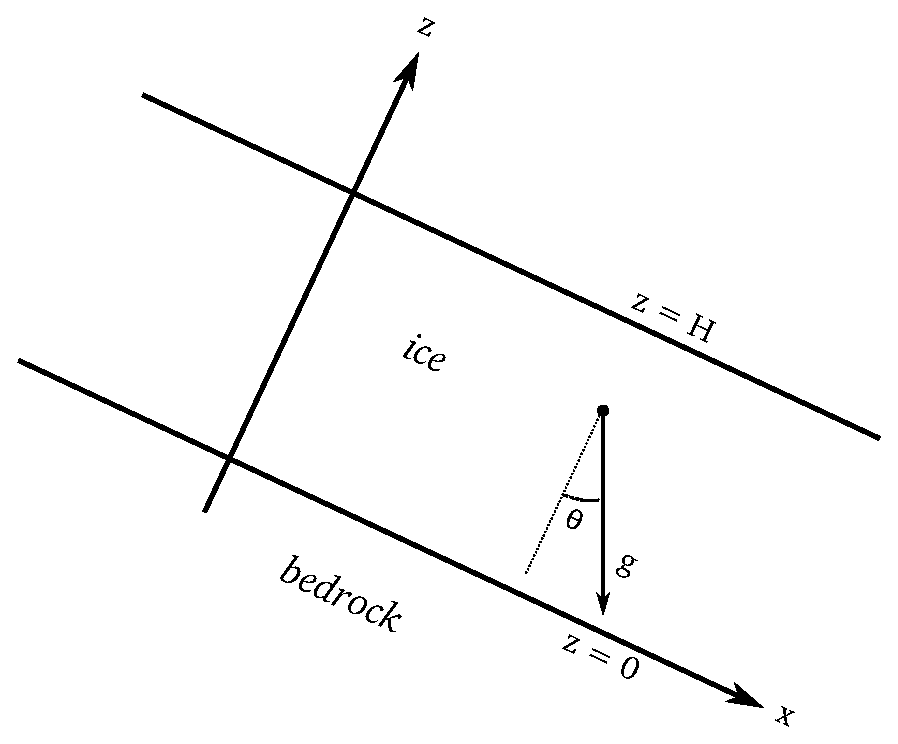
\includegraphics[width=1.0\textwidth]{slab}
\end{column}

\end{columns}

\begin{itemize}
\item for a slab-on-a-slope there is \emph{no variation in} $x$
\item so equations simplify:
\small
\begin{empheq}[box=\fbox]{align}
w_z &= 0 &   0 &= \tau_{11} \notag \\
\tau_{13,z} &= - \rho g \sin\theta &   u_z &= 2 A \tau^2 \tau_{13} \notag \\
p_z &= - \rho g \cos\theta \notag
\end{empheq}
\normalsize
\end{itemize}
\end{frame}


\begin{frame}{slab-on-a-slope 2}

\begin{itemize}
\item add some boundary conditions:
	$$w(\text{base})=0, \qquad p(\text{surface})=0, \qquad u(\text{base})=u_0$$
\item by integrating vertically, get :
  $$w=0, \qquad p = \rho g \cos\theta (H-z), \qquad \tau_{13} = \rho g \sin\theta (H-z)$$
\item and from ``$u_z = 2 A \tau^2 \tau_{13}$'' get
\vspace{-0.05in}
\begin{align*}
u(z) &= u_0 + 2 A (\rho g \sin\theta)^3 \int_0^z (H-z')^3\,dz' \\
     &= u_0 + \frac{1}{2} A (\rho g \sin\theta)^3  \left(H^4 - (H-z)^4\right)
\end{align*}
\end{itemize}

\begin{center}
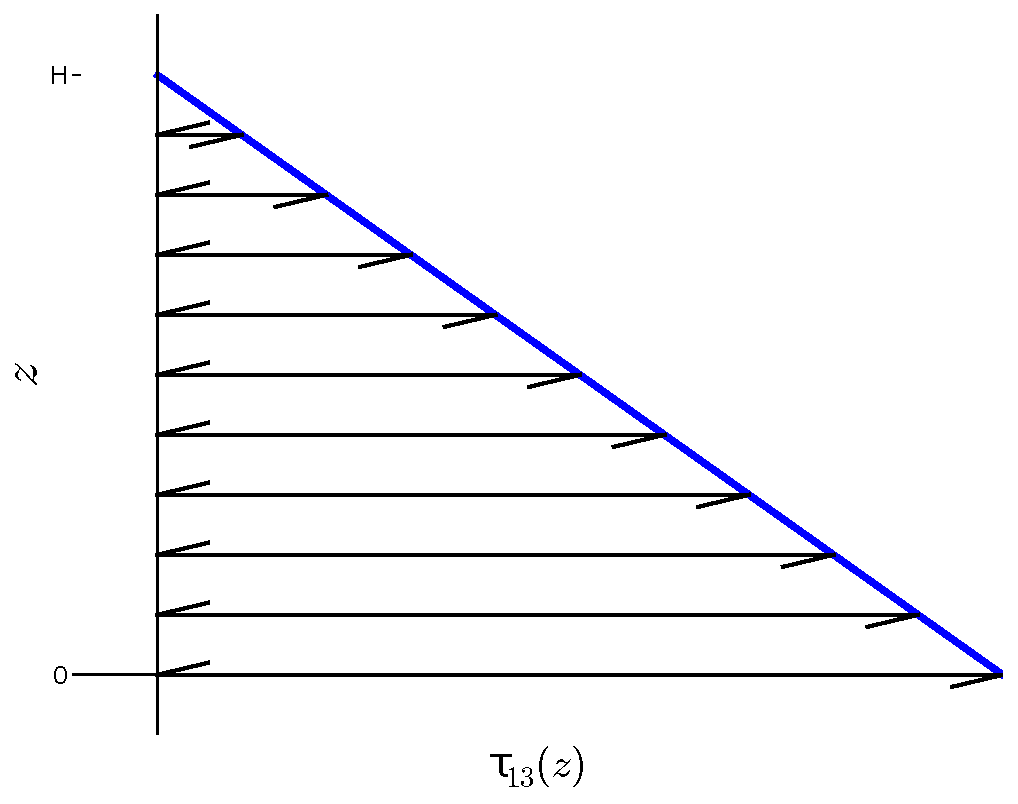
\includegraphics[width=0.4\textwidth]{slabshear}
\end{center}
\end{frame}


\begin{frame}{slab-on-a-slope 3}

\begin{columns}
\begin{column}{0.6\textwidth}
\begin{itemize}
\item do we believe these equations?
\item velocity on last slide (and below) was from a \emph{formula}
\item compare to observations at right
\end{itemize}
\begin{center}
% NOT preserving aspect ratio
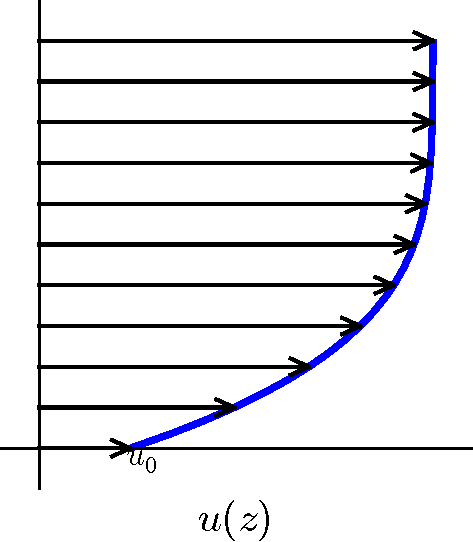
\includegraphics[width=0.6\textwidth,height=0.5\textheight]{slabvel}
\end{center}
\end{column}

\begin{column}{0.4\textwidth}
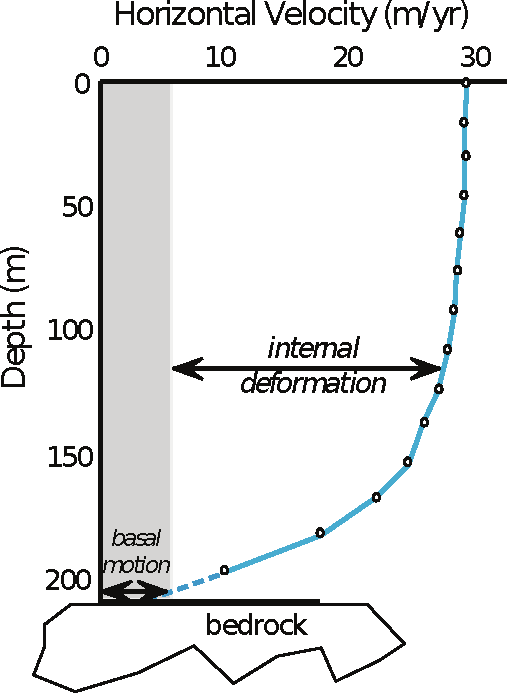
\includegraphics[width=1.0\textwidth]{athabasca_deform}

\medskip
\scriptsize
Velocity profile of the Athabasca Glacier, Canada, derived from inclinometry (Savage and Paterson, 1963)\nocite{SavagePaterson}
\end{column}
\end{columns}
\end{frame}


\begin{frame}{mass continuity}

\small
\begin{itemize}
\item now we know the velocity $u=u(t,x,z)$ \dots so what?
\item suppose our slab has variable thickness $H(t,x)$
\item compute the vertical average of velocity:
	$$\bar u(x,t) = \frac{1}{H}\int_0^{H} u(t,x,z)\,dz$$
\end{itemize}

\begin{columns}
\begin{column}{0.6\textwidth}
\begin{itemize}
\item consider change of area (ice volume in 3D) in the figure:
	$$\frac{dA}{dt} = \int_{x_1}^{x_2} M(x)\,dx + \bar u_1 H_1 - \bar u_2 H_2$$
\item but, assuming width $dx=x_2-x_2$ is small, $A\approx dx\, H$; divide by $dx$ and get
   $$H_t = M - \left(\bar u H\right)_x$$
\item this is a \emph{mass continuity equation}
\item I'll return to this topic \dots
\end{itemize}
\end{column}
\begin{column}{0.4\textwidth}
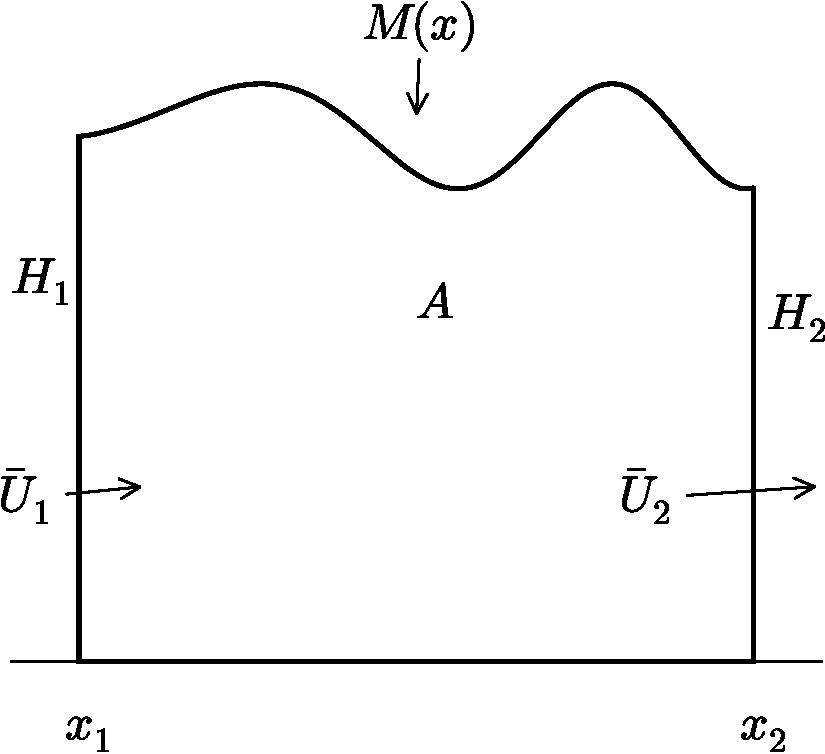
\includegraphics[width=1.0\textwidth]{slabmasscontfig}
\end{column}
\end{columns}
\end{frame}


\begin{frame}{rough explanation of ``shallow ice approximation'' (SIA)}

\small
\begin{itemize}
\item from slab-on-slope velocity formula in $u_0=0$ case (``non-sliding SIA''),
\begin{align*}
\bar u H &= \int_0^H \frac{1}{2} A (\rho g \sin\theta)^3  \left(H^4 - (H-z)^4\right)\,dz \\
	&= \frac{1}{2} A (\rho g \sin\theta)^3  \left(\frac{4}{5} H^5\right) \\
	&= \frac{2}{5} A (\rho g \sin\theta)^3 H^5
\end{align*}
\item note $\sin \theta \approx \tan\theta = - h_x$
\item combine with mass continuity $H_t = M - \left(\bar u H\right)_x$:
  $$H_t = M + \left(\frac{2}{5} (\rho g)^5 A H^5 |h_x|^2 h_x\right)_x.$$
\item I'll return to this topic \dots
\end{itemize}
\end{frame}

% Copyright 2009--2010  Ed Bueler

\section{heat analogy \& numerics}

\subsection{analogy}

\begin{frame}{compare to heat equation}
\label{slide:heatcompare}

\small
\begin{columns}
\begin{column}{0.6\textwidth}
\begin{itemize}
\item recall Newton's law of cooling
	$$\frac{dT}{dt} = -\mu (T-T_{\text{ambient}})$$
where $T$ is temperature and $\mu$ relates to material and geometry of object
\item Newton's law for segments of an insulated rod:
\begin{align*}
\frac{dT_j}{dt} &= -\tilde \mu \left(T_j - \frac{1}{2} (T_{j-1} + T_{j+1}) \right) \\
	&= \frac{\tilde \mu}{2} \left(T_{j-1} - 2 T_j + T_{j+1}\right) 
\end{align*}
(where $\tilde \mu$ is material constant proportional to $\Delta x^{-2}$)
\item this suggests finite difference approximation of a PDE:
	$$T_t = D T_{xx}$$
\end{itemize}
\end{column}
\begin{column}{0.4\textwidth}
\hfill
\includegraphics[width=0.5\textwidth]{pdffigs/coffee}
\vspace{0.7in}
\includegraphics[width=1.0\textwidth]{pdffigs/heatconduction}

%COFFEE: \hfill \tiny (\emph{user:Assassingr, wiki commons image})
%HEAT:  \hfill \tiny (\emph{Christophe Dang Ngoc Chan, wiki commons image})
\end{column}
\end{columns}
\end{frame}


\begin{frame}{compare to heat equation 2}

\small
continuum version:
\begin{columns}
\begin{column}{0.6\textwidth}
\begin{itemize}
\item Fourier rewrote Newton's law as heat flux in continua: $\mathbf{q} = - k \grad u$
\item by conservation of energy, allowing an additional source of heat $f$, get heat equation:
	$$\rho c u_t = f + \Div (k \grad u)$$
\end{itemize}
\end{column}
\begin{column}{0.4\textwidth}
\animategraphics[autoplay,loop,height=2.5cm]{4}{anim/heatmelt}{0}{16}
\end{column}
\end{columns}


\begin{itemize}
\item set $D=k/(\rho c)$ and $M=f/(\rho c)$:
\begin{empheq}[box=\fbox]{equation}
u_t = M + \Div (D\, \grad u) \label{heat}
\end{empheq}
\item this heat equation is a diffusive, time-dependent PDE, \emph{like the SIA model for ice sheets}
\end{itemize}
\end{frame}


\begin{frame}{analogy: SIA versus heat equation}

\begin{itemize}
\item side-by-side comparison:
\begin{center}
\begin{tabular}{cc}
\scriptsize SIA: $H(t,x,y)$ is ice thickness & \scriptsize heat: $u(t,x,y)$ is temperature \normalsize \\
	\boxed{H_t = M + \Div \left({\color{red}\Gamma H^{n+2} |\grad h|^{n-1}}\, \grad h \right)}  &  \boxed{u_t = M + \Div (D\, \grad u)}
\end{tabular}
\end{center}

\medskip
\item we identify the diffusivity in the SIA:
	$$D = {\color{red}\Gamma H^{n+2} |\grad h|^{n-1}}$$
\item non-sliding shallow ice flow \emph{diffuses} the ice because the flow is down the surface gradient

\bigskip
\item some issues with this analogy:
  \begin{itemize}
  \item[$\circ$]  $\grad H\ne \grad h$ when bed is not flat \dots so what?
  \item[$\circ$]  $D$ depends on solution $H(t,x,y)$ \dots how does that complicate the numerical solution method?
  \item[$\circ$]  $D\to 0$ at margin ($H\to 0$) and at dome ($|\grad h|\to 0$) \dots so what?
  \end{itemize}
\item I'll get back to these ``issues'', but now let's get our hands dirty and numerically solve the heat equation
\end{itemize}
\end{frame}


\subsection{finite differences}

\begin{frame}{finite differences for heat equation}

basic ideas of finite differences:
\begin{itemize}
\item for differentiable $f(x)$ and any $\Delta x$, \emph{Taylor} says
\small
	$$f(x+\Delta x) = f(x) + f'(x) \Delta x + \frac{1}{2} f''(x) \Delta x^2 + \frac{1}{3!} f'''(x) \Delta x^3 + \dots$$
\normalsize
\item you can replace ``$\Delta x$'' with other expressions, e.g.:
\small
\begin{align*}
f(x-\Delta x) &= f(x) - f'(x) \Delta x + \frac{1}{2} f''(x) \Delta x^2 - \frac{1}{3!} f'''(x) \Delta x^3 + \dots \\
f(x+2\Delta x) &= f(x) + 2 f'(x) \Delta x + 2 f''(x) \Delta x^2 + \frac{4}{3} f'''(x) \Delta x^3 + \dots
\end{align*}
\normalsize
\item basic finite difference idea for differential equations: \emph{combine expressions like these to approximate derivatives}
\item for all of these notes, grid points have equal spacing $\Delta x$
\end{itemize}
\end{frame}


\begin{frame}{finite differences for heat equation 2}

\begin{itemize}
\item \emph{partial} derivative expressions, for example with $u=u(t,x)$:
\small
\begin{align*}
u_t(t,x) &= \frac{u(t+\Delta t,x) - u(t,x)}{\Delta t} + O(\Delta t), \\
u_t(t,x) &= \frac{u(t+\Delta t,x) - u(t-\Delta t,x)}{2\Delta t} + O(\Delta t^2), \\
u_x(t,x) &= \frac{u(t,x+\Delta x) - u(t,x)}{\Delta x} + O(\Delta x), \\
u_x(t,x) &= \frac{u(t,x+\Delta x) - u(t,x-\Delta x)}{2\Delta x} + O(\Delta x^2), \\
u_{xx}(t,x) &= \frac{u(t,x+\Delta x) - 2 u(t,x) + u(t,x-\Delta x)}{\Delta x^2} + O(\Delta x^2)
\end{align*}
\normalsize
\item sometimes we want a derivative in-between grid points:
\small
	$$u_x(t,x+(\Delta x/2)) = \frac{u(t,x+\Delta x) - u(t,x)}{\Delta x} + O(\Delta x^2)$$
\normalsize
\item ``$+O(\Delta x^2)$'' is better than ``$+O(\Delta x)$'' if $\Delta x$ is a small number
\end{itemize}
\end{frame}


\begin{frame}{explicit scheme for heat equation}
\label{slide:explicit}

\begin{itemize}
\item recall 1D heat equation $u_t = D u_{xx}$
\item the \emph{explicit} scheme using notation $u_j^n \approx u(t_n,x_j)$, so
	$$\frac{u_j^{n+1} - u_j^n}{\Delta t} = D\,\frac{u_{j+1}^n - 2 u_j^n + u_{j-1}^n}{\Delta x^2}$$
\item let $\nu = D \Delta t / (\Delta x)^2$, so
	$$u_j^{n+1} = \nu u_{j+1}^n + (1 - 2 \nu) u_j^n + \nu u_{j-1}^n$$
\end{itemize}

\begin{columns}[b]
\begin{column}{0.70\textwidth}
\begin{itemize}
\item scheme has stencil at right \large $\to$ \normalsize
\item advantage over implicit (later): $u_j^{n+1}$ is determined by \emph{known} quantities at time $t_n$
\bigskip
\end{itemize}
\end{column}
\begin{column}{0.3\textwidth}
\includegraphics[width=1.0\textwidth]{photos/expstencil}
\end{column}
\end{columns}
\end{frame}


\begin{frame}{explicit scheme for heat equation 2}

\begin{itemize}
\item in 2D we write $u_{jk}^n \approx u(t_n,x_j,y_k)$
\item the 2D explicit scheme for the $M=0$ heat equation $u_t = D(u_{xx} + u_{yy})$ is
\small
	$$\frac{u_{jk}^{n+1} - u_{jk}^n}{\Delta t} = D\,\left(\frac{u_{j+1,k}^n - 2 u_{jk}^n + u_{j-1,k}^n}{\Delta x^2} + \frac{u_{j,k+1}^n - 2 u_{jk}^n + u_{j,k-1}^n}{\Delta y^2}\right)$$
\normalsize
\item or, with $\nu^x := D \Delta t / (\Delta x)^2$ and $\nu^y := D \Delta t / (\Delta y)^2$,
\small
\begin{align*}
u_{jk}^{n+1} &= (1 - 2 \nu^x - 2 \nu^y) u_{jk}^n + \nu^x \left(u_{j+1,k}^n + u_{j-1,k}^n\right) + \nu^y \left(u_{j,k+1}^n + u_{j,k-1}^n\right)
\end{align*}
\end{itemize}

\begin{columns}[b]
\begin{column}{0.62\textwidth}
note: new value $u_{jk}^{n+1}$ is \emph{average} (is it?) of five quantities at old time $t_n$ \qquad $\longrightarrow$
\end{column}
\begin{column}{0.38\textwidth}
\includegraphics[width=1.1\textwidth]{photos/exp2dstencil}
\end{column}
\end{columns}
\end{frame}


\begin{frame}{implementation}
\label{slide:heatmatlab}

\minput{heat}

\small
\begin{itemize}
\item solves $u_t = D(u_{xx} + u_{yy})$ on square $-1 < x < 1$, $-1 < y < 1$
\item choice: gaussian initial condition
\item ``colon notation'' removes loops over spatial variables
\item to approximate $u$ on $30\times 30$ spatial grid, with $D=1$ and $N=20$ steps of length $\Delta t = 0.001$,

\texttt{>>  heat(1.0,30,30,0.001,20)}
\end{itemize}
\end{frame}


\begin{frame}{the look of success}

\begin{itemize}
\item solving $u_t = D(u_{xx} + u_{yy})$ on $30\times 30$ grid
\end{itemize}

\bigskip\bigskip
\begin{columns}
\begin{column}{0.5\textwidth}
initial condition $u(0,x,y)$

\bigskip
\begin{center}
\includegraphics[width=1.0\textwidth]{photos/initialheat}
\end{center}
\end{column}
\begin{column}{0.5\textwidth}
approximate solution $u(t,x,y)$ at $t=0.02$ with $\Delta t=0.001$ 

\bigskip
\begin{center}
\includegraphics[width=1.0\textwidth]{photos/finalheat}
\end{center}
\end{column}
\end{columns}
\end{frame}


\begin{frame}{the look of instability}

\begin{itemize}
\item both figures are from solving $u_t = D(u_{xx} + u_{yy})$ on the same $50\times 50$ grid, at same final time and with same $D$, but with slightly different time steps
\end{itemize}

\bigskip
\begin{columns}
\begin{column}{0.5\textwidth}
\begin{center}
\includegraphics[width=1.0\textwidth]{photos/stability}
%$D=1,\Delta t = 0.00064286,\Delta x = \Delta y = 0.04$ so
  $$FIXME: see notes \frac{D\Delta t}{\Delta x^2}= 0.402$$
\end{center}
\end{column}
\begin{column}{0.5\textwidth}
\begin{center}
\includegraphics[width=1.0\textwidth]{photos/instability}
%$D=1,\Delta t = 0.001,\Delta x = \Delta y = 0.04$ so
  $$FIXME: see notes \frac{D\Delta t}{\Delta x^2}= 0.625$$
\end{center}
\end{column}
\end{columns}
\end{frame}


\begin{frame}{why unstable?}
\label{slide:maxprinc}

\begin{itemize}
\item the 1D first-order explicit scheme in the form 
	$$u_j^{n+1} = \nu u_{j+1}^n + (1 - 2 \nu) u_j^n + \nu u_{j-1}^n$$
gives new value $u_j^{n+1}$ as an \emph{average} of old values,
\item but it is only an average if the middle coefficient is positive:\footnote{recommended basic reference for finite differences, including stability: [Morton and Mayers, 2005]\nocite{MortonMayers}}
	$$1 - 2 \nu = 1 - 2 \frac{D\Delta t}{\Delta x^2} \ge 0$$
\item true averaging is always stable because averaged wiggles are smaller than the previous wiggles
\item ``positive coefficients'' is a \emph{sufficient} stability criterion
\item the same thing as a time-step restriction:
	$$\Delta t \le \frac{\Delta x^2}{2 D}$$
\end{itemize}
\end{frame}


\begin{frame}{\textsl{adaptive} implementation: guaranteed stability}

\minput{heatadapt}

\small
\begin{itemize}
\item same as \texttt{heat.m} except it gets the time step from:
	$$\frac{D\Delta t}{(\min\{\Delta x,\Delta y\})^2} \le \frac{1}{4}$$
\end{itemize}\end{frame}


\begin{frame}{alternative instability fix: implicitness}

\begin{columns}[T]
\begin{column}{0.7\textwidth}
\small
\begin{itemize}
\item explicit scheme is only ``conditionally stable'', but there are methods which are stable for \emph{any} positive time step $\Delta t$
\item the simplest such is \emph{first-order implicit} $\to$,
	$$\frac{u_j^{n+1} - u_j^n}{\Delta t} = D\,\frac{u_{j+1}^{n+1} - 2 u_j^{n+1} + u_{j-1}^{n+1}}{\Delta x^2}$$
\item another is \emph{Crank-Nicolson} $\to$; instead of $O(\Delta t,\Delta x^2)$ like first-order explicit and implicit, Crank-Nicolson is $O(\Delta t^2,\Delta x^2)$
\end{itemize}
\end{column}
\begin{column}{0.3\textwidth}
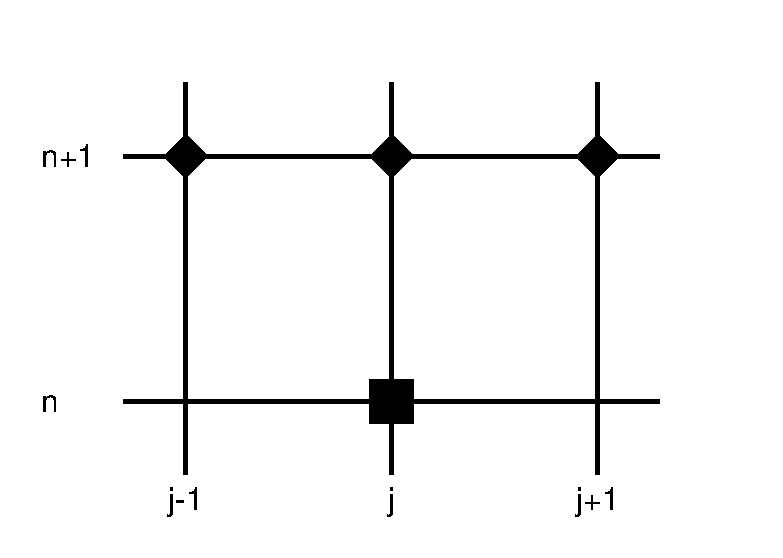
\includegraphics[width=1.2\textwidth]{pdffigs/impstencil}

\bigskip
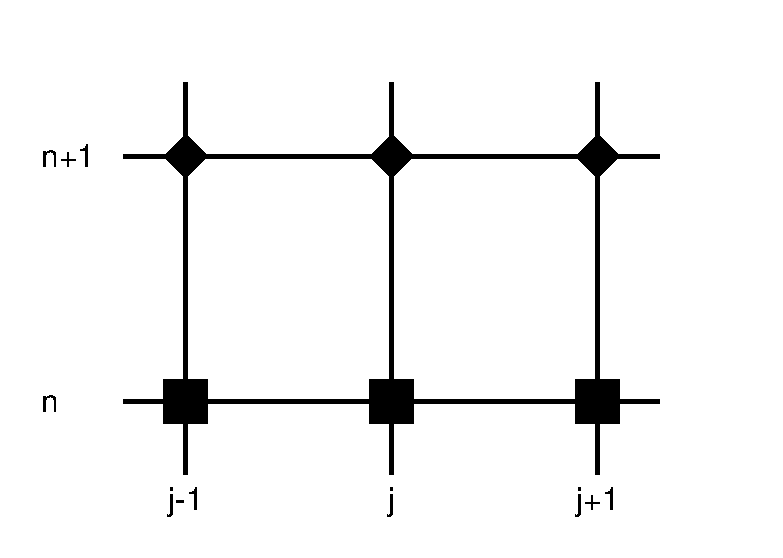
\includegraphics[width=1.2\textwidth]{pdffigs/cnstencil}
\end{column}
\end{columns}

\begin{itemize}
\small
\item \emph{but} for implicit and Crank-Nicolson methods you have to solve systems of equations to take each step
\medskip

\item \scriptsize Donald Knuth has advice for ice sheet modelers: \begin{quote}
\emph{We should forget about small efficiencies, say about 97\% of the time: premature optimization is the root of all evil}.
\end{quote}
\end{itemize}
\end{frame}


\begin{frame}{variable diffusivity and time steps}

\begin{itemize}
  \item recall analogy \qquad (SIA) $\leftrightarrow$ (heat eqn)
  \item the SIA has a diffusivity $D$ which varies in time and space, so by analogy:
  		$$u_t = M + \Div \left(D(t,x,y) \grad \right)$$
  \item the explicit method is conditionally stable with the ``same'' stability condition \emph{if} we evaluate diffusivity $D(t,x,y)$ at \alert{staggered} grid points:
  \scriptsize
\begin{align*}
\Div \left(D(t,x,y) \grad u\right) &\approx \frac{D_{j+1/2,k}(u_{j+1,k} - u_{j,k}) - D_{j-1/2,k}(u_{j,k} - u_{j-1,k})}{\Delta x^2} \\
	&\qquad + \frac{D_{j,k+1/2}(u_{j,k+1} - u_{j,k}) - D_{j,k-1/2}(u_{j,k} - u_{j,k-1})}{\Delta y^2}
\end{align*}
\end{itemize}

\vspace{-0.15in}
\small
\begin{columns}
\begin{column}{0.55\textwidth}
in stencil at right:
\begin{itemize}
\item[] diamonds: $u$
\item[] triangles: $D$
\end{itemize}
\end{column}
\begin{column}{0.45\textwidth}
\begin{center}
\vspace{-0.15in}
\includegraphics[width=1.0\textwidth]{photos/diffstencil}
\end{center}
\end{column}
\end{columns}
\end{frame}


\begin{frame}
  \frametitle{general diffusion equation code}

\minput{diffusion}

\small
\begin{itemize}
\item solves abstract diffusion equation $u_t = \Div \left(D(x,y)\, \grad u\right)$
\item user must supply diffusivity on staggered grid
\end{itemize}
\end{frame}


\subsection{exact solutions}

\begin{frame}{on exact solutions}

\begin{itemize}
\item I am not quite done with the (heat) $\leftrightarrow$ (SIA) analogy
\item \dots I also want to use it to address exact solutions and verification

\bigskip
\item the two senses of ``solution'':
  \begin{itemize}
  \small
  \item[$\circ$] a \emph{solution} $u(t,x,y)$ of the heat equation is a function of time and space for which $u_t = M + \Div (D\, \grad u)$ is true
  \item[$\circ$] a \emph{solution} of the heat equation is a \emph{prediction} of that model
  \normalsize
  \end{itemize}
\item exact solutions are exact predictions of the model, but not exact predictions about nature
\item if we can only \emph{approximately} find solutions of a model then knowing a few exact solutions can help test and maintain the quality of the actual code that does the approximation \dots this is \emph{verification} [Wesseling, 2001]\nocite{Wesseling}
\end{itemize}
\end{frame}


\begin{frame}{exact solutions of heat equation}

\begin{itemize}
\item \emph{many} solutions to the heat equation are known, but one is ``fundamental'' to the time-dependent equation, namely the Green's function
\end{itemize}

\begin{columns}[b]
\begin{column}{0.5\textwidth}
\begin{itemize}
\small
\item as time goes it changes shape by shrinking the output (vertical) axis and simultaneously lengthening the input (horizontal) axis
\item \dots \emph{but otherwise it is the same shape}, so it is self-similar
\item there are solutions of the SIA just like this
\normalsize
\end{itemize}
\end{column}
\begin{column}{0.5\textwidth}
\begin{center}
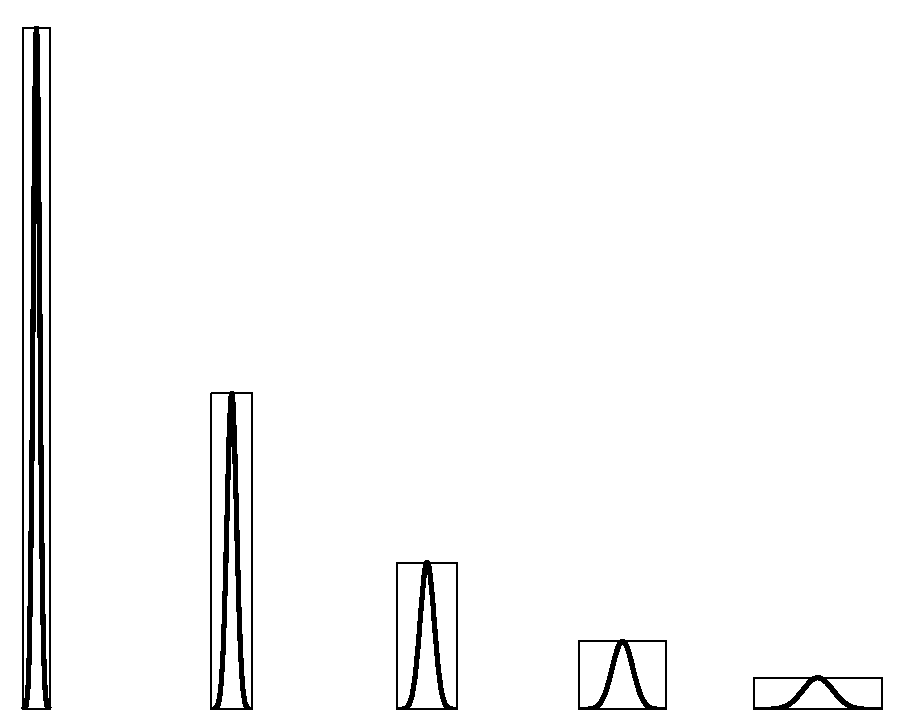
\includegraphics[width=1.0\textwidth]{pdffigs/heatscaling}

\emph{increasing time} \Large $\to$
\end{center}
\end{column}
\end{columns}
\end{frame}


\begin{frame}{finding the Green's function of the heat equation}

\begin{itemize}
\item the best-known way to find the Green's function of the heat equation is by Fourier transform, but we use a method which generalizes to the SIA
\item facts used to find it:
  \begin{itemize}
    \item[$\circ$] the Green's function starts at time $t=0$ with a \emph{delta function} at the origin $r=0$
    \item[$\circ$] the Green's function is angularly-symmetric:  $u$ is a function of the polar coordinate $r = \sqrt{x^2+y^2}$
    \item[$\circ$] calculus says: if $f=f(r)$ then $\grad^2 f = r^{-1} \left(r f'\right)'$
    \item[$\circ$] thus the heat equation in 2D, without additional heat sources, with constant diffusivity $D>0$, and for a function of $r$, is:
   $$u_t = D r^{-1} \left(r u_r\right)_r$$
  \end{itemize}
\item we use above facts to get Green's function by its ``similarity'' properties
\item \emph{but} we do not use the linearity of the heat equation
\end{itemize}
\end{frame}


\begin{frame}{finding a ``similarity'' solution of heat equation}
\label{slide:heatsim}

\small
\begin{itemize}
\item function $u(t,r)$ is replaced by function $\phi$ of one new variable $s$
\item input scaling: $s = t^{-\beta} r$
\item output scaling: $u = t^{-\alpha} \phi(s)$
\item chain rule says:
\begin{align*}
  u_t &= -\alpha t^{-\alpha-1} \phi - \beta t^{-\alpha-\beta-1} r \phi', \qquad u_r = t^{-\alpha-\beta} \phi', \qquad \text{etc.}
\end{align*}
\item so heat equation $u_t = D r^{-1} \left(r u_r\right)_r$ is replaced by:
	$$-\alpha \phi - \beta s \phi' = D s^{-1} t^{-2\beta+1} \left(\phi' + s \phi''\right)$$
\item choose $\boxed{\beta=1/2}$ so equation has no ``$t$'' and further simplify to
   $$-\frac{1}{2} \left[2 \alpha s \phi + s^2 \phi'\right] = D \left(s\, \phi'\right)'$$
\item choose $\boxed{\alpha = 1}$ so that quantity in square brackets simplifies to a derivative: $2 \alpha s \phi + s^2 \phi' = \left(s^2 \phi\right)'$
\end{itemize}
\end{frame}


\begin{frame}{finding a ``similarity'' solution of heat equation 2}

\small
\begin{itemize}
\item simplify and integrate, choose $C=0$, integrate again:
\begin{align*}
  - \frac{1}{2} s^2 \phi &= D\, s\,\phi' + C\\
  \phi' &= - \frac{s}{2D} \phi \\
  \phi(s) &= A e^{-s^2/(4D)}
\end{align*}
\item return to original variables, recalling $s = t^{-\beta} r$:
	$$u(t,r) = A\,t^{-1}\, e^{-r^2/(4Dt)} = A\,t^{-1}\, e^{-(x^2+y^2)/(4Dt)}$$
\item it is a spreading gaussian distribution
\item heat equation is linear so \emph{all} time-dependent solutions of the heat equation are convolutions with this solution \dots which is why it is \emph{fundamental}
\end{itemize}

\begin{center}
\animategraphics[autoplay,loop,height=2cm]{4}{anim/heatmelt}{0}{16}
\end{center}
\end{frame}


\begin{frame}{similarity solutions}

\begin{itemize}
\item \emph{conclusion from previous slides}: similarity variables for heat equation are
	$$s \stackrel{\text{\emph{input scaling}}}{\phantom{\Big|}=\phantom{\Big|}} t^{-\beta} x, \qquad u(t,x) \stackrel{\text{\emph{output scaling}}}{\phantom{\Big|}=\phantom{\Big|}} t^{-\alpha} \phi(s)$$
\item dimension dependence:
	\begin{tabular}{l|ccc}
	               & 1D & 2D & 3D \\ \hline
	input scaling ($t^{-\beta}$)   & $t^{-1/2}$ & $t^{-1/2}$ & $t^{-1/2}$ \\
	output scaling ($t^{-\alpha}$) & $t^{-1/2}$ & $t^{-1}$ & $t^{-3/2}$
	\end{tabular}
\end{itemize}
\begin{columns}
\begin{column}{0.6\textwidth}
\emph{historical note}:  In 1905 Einstein saw that the average distance traveled in time $t$ by particles in thermal motion goes like $\sqrt{t}$.  This is a microscopic explanation of the similarity variable $s = t^{-1/2}x$.
\end{column}
\begin{column}{0.4\textwidth}
\hfill \includegraphics[width=0.8\textwidth]{photos/brownian}
\end{column}
\end{columns}
\end{frame}



\section{shallow ice sheets}

\begin{frame}{slow, non-Newtonian, some basal slip, and shallow}

\begin{itemize}
\item ice sheets have four outstanding properties \emph{as fluids}:
  \begin{enumerate}
  \item slow
  \item non-Newtonian
  \item contact slip (sometimes)
  \item shallow
  \end{enumerate}
\end{itemize}
\end{frame}


\begin{frame}{regarding ``shallow''}

\begin{itemize}
\item below in \alert{red} is a no-vertical-exaggeration cross section of Greenland at $71^\circ$
\small
  \begin{itemize}
  \item[$\circ$] green and blue: standard vertically-exaggerated cross section
  \end{itemize}
  \begin{center}
    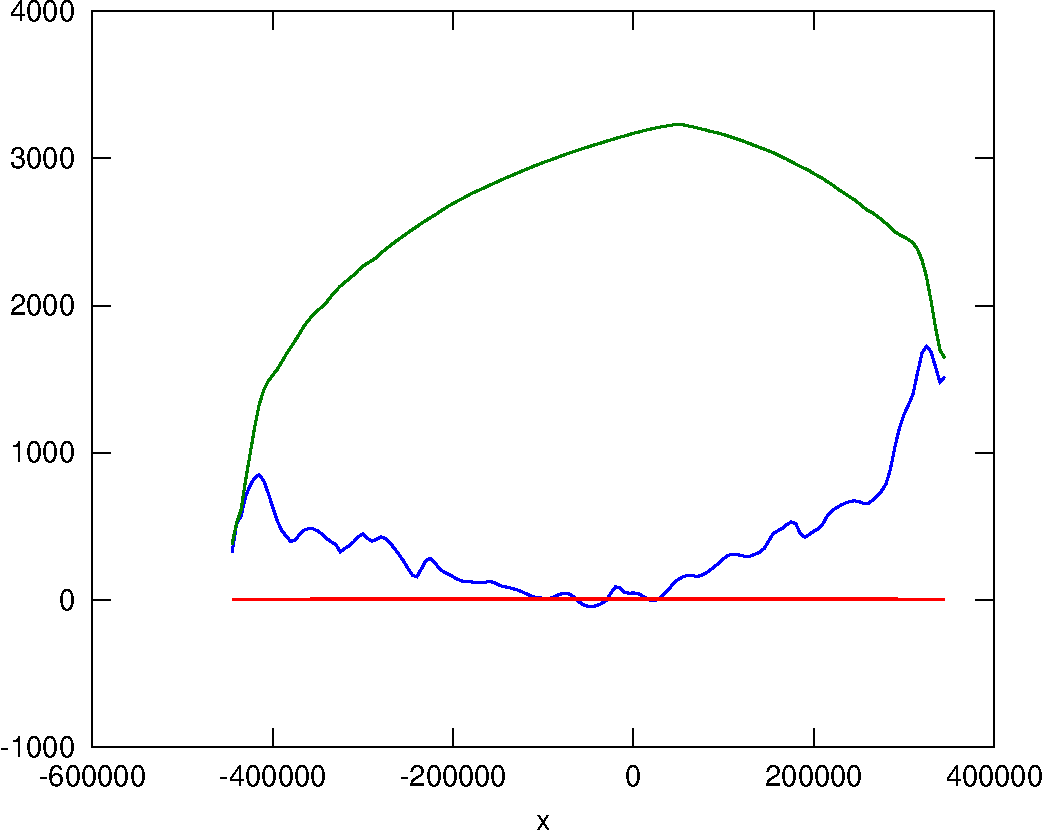
\includegraphics[width=0.6\textwidth]{green_transect}
  \end{center}
\item you can scale Stokes equation using smallness of $\eps = [H]/[L]$, where $[H]$ is a typical thickness of an ice sheet and $[L]$ is a typical horizontal dimension, \dots
\end{itemize}
\end{frame}


\subsection{shallow ice approx (SIA)}

\begin{frame}{non-sliding, isothermal shallow ice approximation = (SIA)}

a model which applies to
\begin{itemize}
\item shallow grounded ice sheets
\item on not-too-rough bed topography,
\item whose flow is not dominated by sliding and/or liquid water at the base or margin
\end{itemize}

\begin{center}
  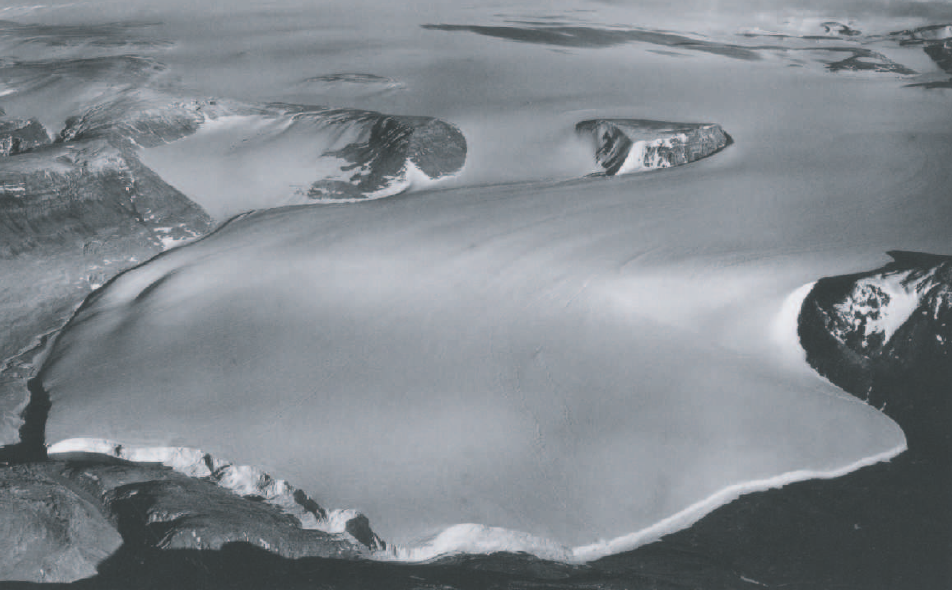
\includegraphics[width=0.65\textwidth]{polaris}

\tiny ``Polaris Glacier,'' northwest Greenland, photo 122, Post \& LaChapelle (2000)
\end{center}

\end{frame}


\begin{frame}{SIA velocity equation}

\begin{itemize}
\item \small here we ``derive'' the SIA by the simple slogan:\normalsize

\begin{center}
\emph{the SIA uses the formulas from slab-on-a-slope}
\end{center}
\item shear stress approximation:
	$$(\tau_{13},\tau_{23}) \approx - \rho g (h-z) \nabla h$$
\item let $\mathbf{U} = (u,v)$, the horizontal velocity
\item we further approximate
\begin{align*}
\mathbf{U}_z &\approx 2 A |(\tau_{13},\tau_{23})|^{n-1} (\tau_{13},\tau_{23}) \\
     &= - 2 A (\rho g)^n (h-z)^n |\nabla h|^{n-1} \nabla h
\end{align*}
\item by integrating vertically, in the non-sliding case,
    $$\mathbf{U} = - \frac{2 A (\rho g)^n}{n+1} \left[H^{n+1} - (h-z)^{n+1}\right] |\nabla h|^{n-1} \nabla h$$
\item but mass continuity remains, $H_t = M - \left(\overline{\mathbf{U}} H\right)_x$
\end{itemize}
\end{frame}


\begin{frame}{SIA thickness equation}

\begin{itemize}
\item combine last two equations on last slide
\item get the non-sliding, isothermal shallow ice approximation for thickness changes:
\begin{empheq}[box=\fbox]{equation*}
H_t = M + \Div \left(\Gamma H^{n+2} |\grad h|^{n-1} \grad h \right)
\end{empheq}

\vspace{-2mm}
  \begin{itemize}
  \item[$\circ$] where $H$ is ice thickness, $h$ is ice surface elevation, $b$ is bed elevation ($h=H+b$)
  \item[$\circ$] $M$ combines surface and basal mass (im)balance:

     accumulation if $M>0$, ablation if $M<0$
  \item[$\circ$] $n$ is the exponent in the Glen flow law
  \item[$\circ$] $\Gamma = 2 A (\rho g)^n / (n+2)$ is a positive constant
  \end{itemize}
\end{itemize}
\end{frame}


\begin{frame}{SIA thickness equation 2}

\begin{itemize}
\item numerically solve this equation
\begin{empheq}[box=\fbox]{equation}
H_t = M + \Div \left(\Gamma H^{n+2} |\grad h|^{n-1} \grad h \right) \label{sia}
\end{empheq}
and you've got a usable model for \dots \emph{the Barnes ice cap} (Mahaffy, 1976)
\end{itemize} 
\medskip

\begin{columns}
\begin{column}{0.5\textwidth}
\noindent good questions:
\begin{enumerate}
\item where does equation (1) come from?
\item how to solve it numerically?
\item how to \emph{think} about it?
\end{enumerate}  
\end{column}

\begin{column}{0.5\textwidth}
\begin{center}
  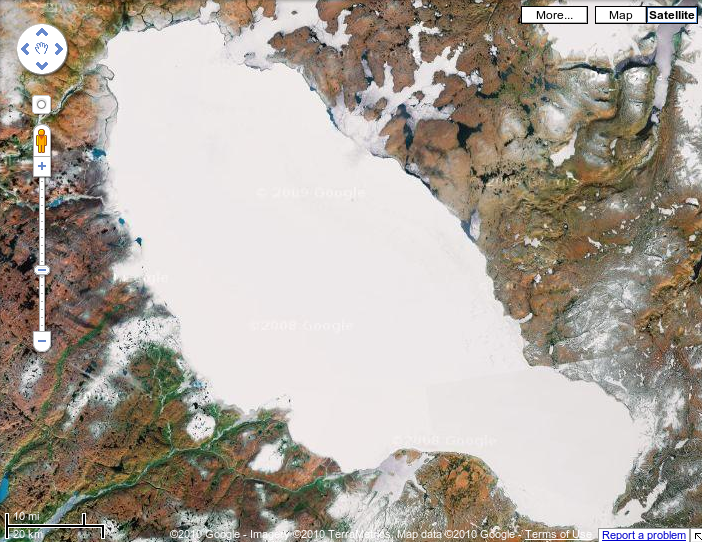
\includegraphics[width=0.8\textwidth]{barnes}
\end{center}
\end{column}
\end{columns}
\end{frame}


\subsection{analogy w heat equation}

\begin{frame}{heat equation}

\small
\begin{columns}
\begin{column}{0.6\textwidth}
\begin{itemize}
\item for understanding the SIA, recall the heat equation describing conduction
\item here's one quick way to derive it \dots
\item Newton's law of cooling for each segment of the rod:
\begin{align*}
\frac{dT_j}{dt} &= - C \left(T_j - \frac{1}{2} (T_{j-1} + T_{j+1}) \right) \\
	&= \frac{C}{2} \left(T_{j-1} - 2 T_j + T_{j+1}\right) 
\end{align*}
\item the limit as segments shrink $\Delta x\to 0$:
	$$T_t = D T_{xx}$$
\item $D=$ diffusivity, with units $\text{m}^2\,\text{s}^{-1}$
\item $T_{xx}>0 \implies T(t)$ decreases
\item $T_{xx}<0 \implies T(t)$ increases
\item so $T(x)$ becomes smoother with time
\end{itemize}
\end{column}

\begin{column}{0.4\textwidth}
\hfill
%\includegraphics[width=0.5\textwidth]{coffee}
\vspace{0.3in}
\includegraphics[width=1.0\textwidth]{heatconduction}
\end{column}
\end{columns}
\end{frame}


\begin{frame}{more complete heat equation}

\small
\begin{columns}
\begin{column}{0.6\textwidth}
\begin{itemize}
\item $T(t,x,y)$ is temperature in a 2D object at position $x,y$ and time $t$
\item Fourier rewrote Newton's law as a rule for heat flux: $\mathbf{q} = - k \grad T$
\item allow an additional heat source $f$
\item coefficients: $\rho$ is density, $c$ is specific heat, $k$ is conductivity
  \begin{itemize}
  \item[$\circ$] let's assume $\rho$, $c$ are constant
  \end{itemize}
\item by conservation of energy:
	$$\rho c T_t = f + \Div (k \grad T)$$
\end{itemize}
\end{column}
\begin{column}{0.4\textwidth}
\animategraphics[autoplay,loop,height=2.5cm]{4}{anim/heatmelt}{0}{16}
\end{column}
\end{columns}

\begin{itemize}
\item define the diffusivity $D=k/(\rho c)$ and also $F := f/(\rho c)$
\item for 2D object (e.g.~a plate), the heat equation:
\begin{equation}
T_t = F + \Div (D\, \grad T) \label{heat}
\end{equation}
\item the temperature $T$ solves a \emph{diffusive, time-evolving partial differential equation (PDE)} \dots just like thickness $H$ in SIA
\end{itemize}
\end{frame}


\begin{frame}{analogy: SIA versus heat equation}

\begin{itemize}
\item side-by-side comparison:
\begin{center}
\begin{tabular}{cc}
\scriptsize SIA:\, $H(t,x,y)$ is ice thickness & \scriptsize heat: $T(t,x,y)$ is temperature \normalsize \\
	\boxed{H_t = M + \Div \left({\color{red}\Gamma H^{n+2} |\grad h|^{n-1}}\, \grad h \right)}  &  \boxed{T_t = F + \Div (D\, \grad T)}
\end{tabular}
\end{center}

\medskip
\item we identify the diffusivity in the SIA:
	$$D = {\color{red}\Gamma H^{n+2} |\grad h|^{n-1}}$$
\item \emph{non-sliding shallow ice flow \alert{diffuses} the ice sheet}
\item some issues with this analogy:
  \begin{itemize}
  \item[$\circ$]  $D$ depends on solution $H(t,x,y)$
  \item[$\circ$]  $D\to 0$ at margin, where $H\to 0$
  \item[$\circ$]  $D\to 0$ at divides/domes, where $|\grad h|\to 0$
  \end{itemize}
\end{itemize}
\end{frame}


\subsection{finite difference numerics}

\begin{frame}{basic ideas of finite differences}

\begin{itemize}
\item numerical schemes for heat equation are good start for SIA
\item for differentiable $f(x)$ and any $\Delta$, \emph{Taylor's theorem} says
	$$f(x+\Delta) = f(x) + f'(x) \Delta + \frac{1}{2} f''(x) \Delta^2 + \frac{1}{3!} f'''(x) \Delta^3 + \dots$$
\normalsize
\item you can replace ``$\Delta$'' by its multiples, e.g.:
\small
\begin{align*}
f(x-\Delta) &= f(x) - f'(x) \Delta + \frac{1}{2} f''(x) \Delta^2 - \frac{1}{3!} f'''(x) \Delta^3 + \dots \\
f(x+2\Delta) &= f(x) + 2 f'(x) \Delta + 2 f''(x) \Delta^2 + \frac{4}{3} f'''(x) \Delta^3 + \dots
\end{align*}
\normalsize
\item basic finite difference idea:
\begin{quote}
\emph{combine expressions like these to give approximations of derivatives from values of $f(x)$ on a grid}
\end{quote}
\end{itemize}
\end{frame}


\begin{frame}{finite differences for partial derivatives}

\begin{itemize}
\item we want partial derivative expressions, for example with some function $u=u(t,x)$:
\small
\begin{align*}
u_t(t,x) &= \frac{u(t+\Delta t,x) - u(t,x)}{\Delta t} + O(\Delta t), \\
u_t(t,x) &= \frac{u(t+\Delta t,x) - u(t-\Delta t,x)}{2\Delta t} + O(\Delta t^2), \\
u_x(t,x) &= \frac{u(t,x+\Delta x) - u(t,x)}{\Delta x} + O(\Delta x), \\
u_{xx}(t,x) &= \frac{u(t,x+\Delta x) - 2 u(t,x) + u(t,x-\Delta x)}{\Delta x^2} + O(\Delta x^2)
\end{align*}
\normalsize
\item sometimes we want a derivative in-between grid points:
\small
	$$u_x(t,x+(\Delta x/2)) = \frac{u(t,x+\Delta x) - u(t,x)}{\Delta x} + O(\Delta x^2)$$
\normalsize
\item ``$+O(\Delta^2)$'' is better than ``$+O(\Delta)$'' if $\Delta$ is a small number
\end{itemize}
\end{frame}


\begin{frame}{explicit scheme for heat equation}
\label{slide:explicit}

\begin{itemize}
\item recall 1D heat equation $T_t = D T_{xx}$
\item an \emph{explicit} scheme:
\small
	$$\frac{T(t+\Delta t,x) - T(t,x)}{\Delta t} = D\,\frac{T(t,x+\Delta x) - 2 T(t,x) + T(t,x-\Delta x)}{\Delta x^2}$$
\normalsize
\item the difference between the equation $T_t = D T_{xx}$ and the scheme is $O(\Delta t,\Delta x^2)$
\item notation: $(t_n,x_j)$ and $T_j^n \approx T(t_n,x_j)$
\item let $\mu = D \Delta t / (\Delta x)^2$, so
\small
	$$T_j^{n+1} = \mu T_{j+1}^n + (1 - 2 \mu) T_j^n + \mu T_{j-1}^n$$
\normalsize
\end{itemize}
\begin{columns}
\begin{column}{0.55\textwidth}
\begin{itemize}
\item scheme has stencil at right \large $\to$ \normalsize
\end{itemize}
\end{column}
\begin{column}{0.45\textwidth}
\includegraphics[width=0.7\textwidth]{expstencil}
\end{column}
\end{columns}
\end{frame}


\begin{frame}{explicit scheme in two space dimensions}

\begin{itemize}
\item recall heat equation in 2D: $T_t = D(T_{xx} + T_{yy})$
\item in two spatial variables we write $T_{jk}^n \approx T(t_n,x_j,y_k)$
\item so the 2D explicit scheme is
\small
	$$\frac{T_{jk}^{n+1} - T_{jk}^n}{\Delta t} = D\,\left(\frac{T_{j+1,k}^n - 2 T_{jk}^n + T_{j-1,k}^n}{\Delta x^2} + \frac{T_{j,k+1}^n - 2 T_{jk}^n + T_{j,k-1}^n}{\Delta y^2}\right)$$
\end{itemize}

\bigskip
\begin{center}
\includegraphics[width=0.35\textwidth]{exp2dstencil}
\end{center}
\end{frame}


\begin{frame}{implementation}
\label{slide:heatmatlab}

\minput{heat}

\small
\begin{itemize}
\item solves $T_t = D(T_{xx} + T_{yy})$ on square $-1 < x < 1$, $-1 < y < 1$
\item uses gaussian initial condition: $T(0,x,y) = e^{-30 r^2}$
\item uses ``colon notation'' to remove loops over spatial variables
\item \texttt{>>  heat(1.0,30,30,0.001,20)}

approximates $T$ on $30\times 30$ spatial grid, with $D=1$ and $N=20$ steps of $\Delta t = 0.001$
\end{itemize}
\end{frame}


\begin{frame}{the look of success}

\begin{itemize}
\item solving $T_t = T_{xx} + T_{yy}$ on $30\times 30$ grid
\end{itemize}

\bigskip
\begin{columns}
\begin{column}{0.5\textwidth}
initial condition $T(0,x,y)$

\phantom{foo}

\bigskip
\begin{center}
\includegraphics[width=1.0\textwidth]{initialheat}
\end{center}
\end{column}
\begin{column}{0.5\textwidth}
approximate solution $T(t,x,y)$ at $t=0.02$ with $\Delta t=0.001$ 

\bigskip
\begin{center}
\includegraphics[width=1.0\textwidth]{finalheat}
\end{center}
\end{column}
\end{columns}
\end{frame}


\begin{frame}{the look of instability}

\begin{itemize}
\item figures below are from solving $T_t = T_{xx} + T_{yy}$ on the same space grid, but with slightly different time steps
\end{itemize}

\bigskip\bigskip
\begin{columns}
\begin{column}{0.5\textwidth}
\begin{center}
\includegraphics[width=1.0\textwidth]{stability}

$$\frac{D\Delta t}{\Delta x^2}= 0.2$$
\end{center}
\end{column}
\begin{column}{0.5\textwidth}
\begin{center}
\includegraphics[width=1.0\textwidth]{instability}

$$\frac{D\Delta t}{\Delta x^2}= 0.4$$
\end{center}
\end{column}
\end{columns}
\end{frame}


\begin{frame}{avoid the instability}

\begin{itemize}
\item recall 1D explicit scheme has form 
	$$T_j^{n+1} = \mu T_{j+1}^n + (1 - 2 \mu) T_j^n + \mu T_{j-1}^n$$
\item thus the new value $T_j^{n+1}$ is an \emph{average} of the old values, \emph{if the middle coefficient is positive}:
	$$1 - 2 \mu \ge 0 \quad \iff \quad  \frac{D\Delta t}{\Delta x^2} \le \frac{1}{2} \quad \iff \quad \Delta t \le \frac{\Delta x^2}{2 D}$$
\item averaging is always stable because averaged wiggles are always smaller than the original wiggles
\item this condition is a sufficient \emph{stability criterion}
\item \emph{the result was unstable because the time step was too big}
\item in 2D case with $\Delta x= \Delta y$ the condition is
	$$\frac{D\Delta t}{\Delta x^2} \le \frac{1}{4}$$
\end{itemize}
\end{frame}


\begin{frame}{\textsl{adaptive} implementation: guaranteed stability}

\scriptsize
\minput{heatadapt}
\normalsize

\begin{itemize}
\item same as \texttt{heat.m} except

\begin{center}
\emph{choose time step from stability criterion}
\end{center}
\end{itemize}\end{frame}


\begin{frame}{alternative instability fix: implicitness}

\begin{itemize}
\item explicit scheme is only ``conditionally stable''
  \begin{itemize}
  \item[$\circ$] the adaptive implementation uses the condition
  \end{itemize}
\item there are \alert{implicit} methods which are stable for \emph{any} $\Delta t$
\item an implicit scheme for the heat equation is \emph{Crank-Nicolson}
  \begin{itemize}
  \item[$\circ$] it has smaller error too: $O(\Delta t^2,\Delta x^2)$
  \end{itemize}
\item \emph{but} you have to solve systems of equations at each time step
\item in nonlinear case you may end up spending much more programmer time to implement implicit methods
  \begin{itemize}
  \item[$\circ$] this can impose a big opportunity cost
  \end{itemize}
\vspace{5mm}

\item \small Donald Knuth has advice for ice sheet modelers: \begin{quote}
\emph{We should forget about small efficiencies \dots: premature optimization is the root of all evil}.
\end{quote}
\end{itemize}
\end{frame}


\begin{frame}{variable diffusivity}

\begin{itemize}
  \item recall the analogy: \qquad (SIA) $\leftrightarrow$ (heat eqn)
  \item the SIA has a diffusivity $D(x,y)$ which varies in space
  \item and it has both $H$ and $h=H+b$
  \item so consider a more general heat equation:
\begin{equation}
T_t = F + \Div \left(D\, \grad (T+b)\right) \tag{$\ast$}
\end{equation}
  \item the best explicit method for $(\ast)$ evaluates diffusivity $D$ at \alert{staggered} grid points:
  \scriptsize
\begin{align*}
\Div \left(D \grad X\right) &\approx \frac{D_{j+1/2,k}(X_{j+1,k} - X_{j,k}) - D_{j-1/2,k}(X_{j,k} - X_{j-1,k})}{\Delta x^2} \\
	&\qquad + \frac{D_{j,k+1/2}(X_{j,k+1} - X_{j,k}) - D_{j,k-1/2}(X_{j,k} - X_{j,k-1})}{\Delta y^2}
\end{align*}
\end{itemize}

\vspace{-0.15in}
\small
\begin{columns}
\begin{column}{0.55\textwidth}
\begin{itemize}
\item best = just as stable as previous
\item in stencil at right:
  \begin{itemize}
  \item[] diamonds: $X = T+b$
  \item[] triangles: $D$
  \end{itemize}
\end{itemize}
\end{column}
\begin{column}{0.45\textwidth}
\begin{center}
\includegraphics[width=0.6\textwidth]{diffstencil}
\end{center}
\end{column}
\end{columns}
\end{frame}


\begin{frame}
  \frametitle{general diffusion equation code}

\minputtiny{diffusion}

\small
\begin{itemize}
\item solves abstract diffusion equation $T_t = \Div \left(D \, \grad (T + b)\right)$
\item user supplies diffusivity $D$ on staggered grid
\end{itemize}
\end{frame}


\subsection{solutions}

\begin{frame}{exact solution of heat equation}

\begin{itemize}
\item before getting to ice flow, one more heat equation topic \dots
\vspace{5mm}

\item many \emph{exact} solutions to the heat equation are known
\item I'll show the ``Green's function''
\item \dots also known as ``heat kernel''
\item it starts at time $t=0$ with a ``delta function'' of heat at the origin $x=0$ and then it spreads out over time
\item we find it by a method which generalizes to the SIA
\end{itemize}
\end{frame}


\begin{frame}{Green's function of heat equation}

\begin{itemize}
\item the solution is ``self-similar'' over time
\item with time it changes shape by
  \begin{itemize}
  \item[$\circ$] shrinking the output (vertical) axis and
  \item[$\circ$] lengthening the input (horizontal) axis
  \end{itemize}
\item \dots but otherwise it is the same shape
\item the integral over $x$ is independent of time
\end{itemize}

\begin{center}
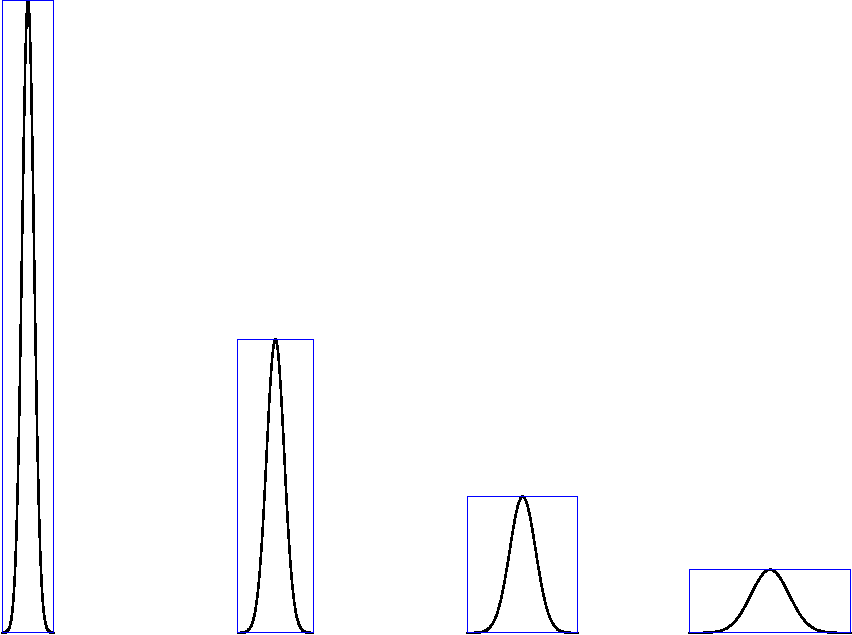
\includegraphics[width=0.5\textwidth]{heatscaling}

\emph{increasing time} \Large $\to$
\end{center}
\end{frame}


\begin{frame}{similarity solutions}

\begin{itemize}
\item Green's function of 1D heat equation ( $T_t=D T_{xx}$ ) is
	$$T(t,x) = C\, t^{-1/2} e^{-x^2/(4Dt)}$$
\item ``similarity'' variables for 1D heat equation are
	$$s \stackrel{\text{\emph{input scaling}}}{\phantom{\Big|}=\phantom{\Big|}} t^{-1/2} x, \qquad u(t,x) \stackrel{\text{\emph{output scaling}}}{\phantom{\Big|}=\phantom{\Big|}} t^{-1/2} \phi(s)$$
\end{itemize}
\begin{columns}
\begin{column}{0.6\textwidth}
\begin{itemize}
\item \emph{historical note}:  in 1905 Einstein saw that the average distance traveled by particles in thermal motion scales like $\sqrt{t}$, so $s = t^{-1/2}x$ is an invariant
\end{itemize}
\end{column}
\begin{column}{0.4\textwidth}
\begin{center}
\includegraphics[width=1.0\textwidth]{brownian}
\end{center}
\end{column}
\end{columns}

\end{frame}


\subsection{solving the SIA}

\begin{frame}{similarity solution to SIA}

\begin{itemize}
\item jump forward to 1981
\item P.~Halfar found the similarity solution of the SIA in the case of flat bed and no surface mass balance
\item Halfar's 2D solution for Glen flow law with $n=3$ has scalings
	$$s \stackrel{\text{\emph{input scaling}}}{\phantom{\Big|}=\phantom{\Big|}} t^{-1/18} r, \qquad H(t,r) \stackrel{\text{\emph{output scaling}}}{\phantom{\Big|}=\phantom{\Big|}} t^{-1/9} \phi(s)$$
\item so: the nonlinear diffusion of the SIA quickly slows down the rate of change of the profile as the shape flattens out
\end{itemize}
\end{frame}


\begin{frame}{Halfar solution to the SIA: the movie}
\label{slide:plothalfar}

\animategraphics[autoplay,loop,height=7.0cm]{4}{anim/halfar}{0}{26}

\par
\scriptsize 
frames from $t=4$ months to $t = 10^6$ years, equal spaced in \emph{exponential} time
\end{frame}


\begin{frame}{Halfar solution to the SIA: the formula}

\begin{itemize}
\item for $n=3$ the solution formula is:
  $$H(t,r) = H_0 \left(\frac{t_0}{t}\right)^{1/9} \left[1 - \left(\left(\frac{t_0}{t}\right)^{1/18} \frac{r}{R_0}\right)^{4/3}\right]^{3/7}$$
\item the ``characteristic time'' is
  $$t_0 = \frac{1}{18 \Gamma} \left(\frac{7}{4}\right)^3 \frac{R_0^4}{H_0^{7}}$$
if $H_0$, $R_0$ are central height and ice cap radius at $t=t_0$
\item you choose $H_0$ and $R_0$ and then determine $t_0$
\item it is a simple formula to use for verification!
\end{itemize}
\end{frame}


\begin{frame}{is the Halfar solution \emph{good for any modelling}?}

\begin{itemize}
\item John Nye and others (2000) compared long-time consequences of different flow laws for the Mars polar caps
\item they evaluated $\text{CO}_2$ ice versus $\text{H}_2\text{O}$ ice parameters
\item \dots by comparing long-time behavior of the Halfar solutions
\item conclusions:
  \begin{quote}
  \dots none of the three possible [$\text{CO}_2$] flow laws will allow a 3000-m cap, the thickness suggested by stereogrammetry, to survive for $10^7$ years, indicating that the south polar ice cap is probably not composed of pure $\text{CO}_2$ ice \dots the south polar cap probably consists of water ice, with an unknown admixture of dust.
  \end{quote}
\end{itemize}

\end{frame}


\begin{frame}{on ``degenerate'' diffusivity}

\begin{itemize}
\item recall that the SIA is
\small
	$$H_t = M + \Div \left(D\, \grad h \right) \quad \text{where} \quad D = \Gamma H^{n+2} |\grad h|^{n-1}$$
\normalsize
\item thus the diffusivity ``degenerates'', $D \to 0$, when either $H\to 0$ or $\grad h \to 0$
\item summary:
\small
\begin{tabular}{l|c|c}
 & why $D\to 0$ & so what? \\ \hline
domes    & $\grad h \to 0$ & \begin{tabular}{c}
$H$ and $\grad h$ are continuous \\ but $\grad^2 h$ is singular
\end{tabular} \\ \hline
margins  & $H \to 0$       & \begin{tabular}{c}
$H$ is continuous \\ but $\grad h$ is singular
\end{tabular}
\end{tabular}
\normalsize
\item in terms of numerical error, margin is worse than dome
\item degenerate diffusion equations are automatically free boundary problems
\end{itemize}
\end{frame}


\begin{frame}
  \frametitle{computing diffusivity in SIA}

\begin{itemize}
\item for numerical stability we compute $D = \Gamma H^{n+2} |\grad h|^{n-1}$ on the staggered grid
\item various schemes proposed
\item all schemes involve
  \begin{itemize}
  \item[$\circ$] averaging $H$
  \item[$\circ$] differencing $h$
  \item[$\circ$] in a ``balanced'' way, for better accuracy,
  \end{itemize}
to get the diffusivity on staggered grid
\end{itemize}

\begin{columns}
\begin{column}{0.65\textwidth}
\begin{itemize}
\item Mahaffy's scheme has stencil \large $\to$ \normalsize
\end{itemize}
\end{column}

\begin{column}{0.35\textwidth}
  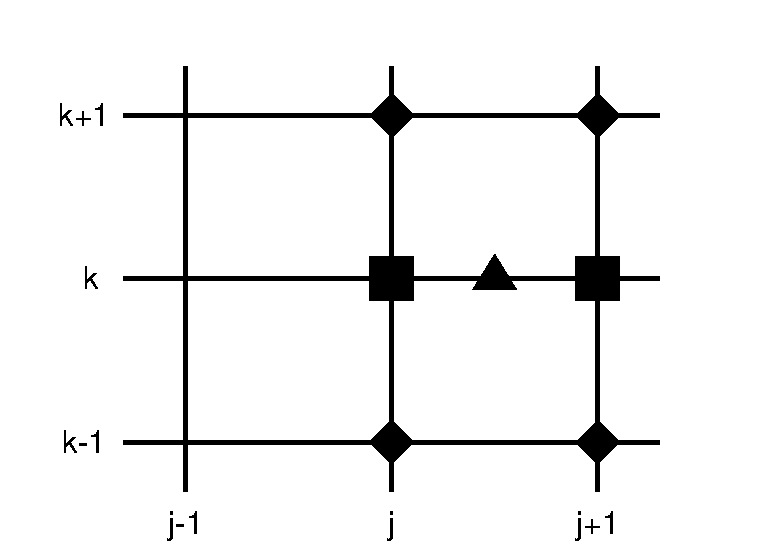
\includegraphics[width=1.0\textwidth]{mahaffystencil}
\end{column}
\end{columns}
\end{frame}


\begin{frame}
  \frametitle{SIA implementation: flat bed case}

\minputtiny{siaflat}

\end{frame}


\begin{frame}{verification of numerical ice flow codes}
\begin{itemize}
\item how do we make sure a numerical scheme is correct?

\vspace{5mm}
\item how do we make sure an \emph{implemented} numerical scheme is correct?
  \begin{itemize}
  \item[$\circ$] \emph{technique} 1: don't make any mistakes
  \item[$\circ$] \emph{technique} 2: compare your model with others, and hope that the outliers are the ones with errors
  \item[$\circ$] \emph{technique} 3: build-in a comparison to an exact solution, and actually measure the numerical error
  \end{itemize}

\vspace{5mm}
\item technique 3 is called \alert{verification}
\end{itemize}
\end{frame}


\begin{frame}{where to get exact solutions for ice flow models?}

\small
\begin{itemize}
  \item textbook: Greve and Blatter (2009)
  \item similarity solutions to SIA (Halfar 1983; Bueler et al 2005)
  \item manufactured solutions to thermo-coupled SIA (Bueler et al 2007)
  \item flowline and cross-flow SSA solutions (van der Veen, 1985; Schoof, 2006)
  \item flowline Blatter solutions (Glowinski and Rappaz 2003)
  \item flowline Stokes solutions for constant viscosity (Ladyzhenskaya 1963; Balise and Raymond 1985)
  \item manufactured solutions to the Stokes equations (Sargent and Fastook 2010; Jouvet and Rappaz 2011)
\end{itemize}
\end{frame}


\begin{frame}[fragile]
\frametitle{verifying SIA code vs Halfar}
\label{slide:verifysia}

\begin{columns}
\begin{column}{0.6\textwidth}
test program \texttt{verifysia.m} calls \texttt{siaflat.m}

\scriptsize
\begin{verbatim}
octave:40> verifysia(20)
average abs error            = 22.310
maximum abs error            = 227.849
octave:41> verifysia(40)
average abs error            = 9.490
maximum abs error            = 241.470
octave:42> verifysia(80)
average abs error            = 2.800
maximum abs error            = 155.796
octave:43> verifysia(160)
average abs error            = 1.059
maximum abs error            = 109.466
\end{verbatim}
\normalsize

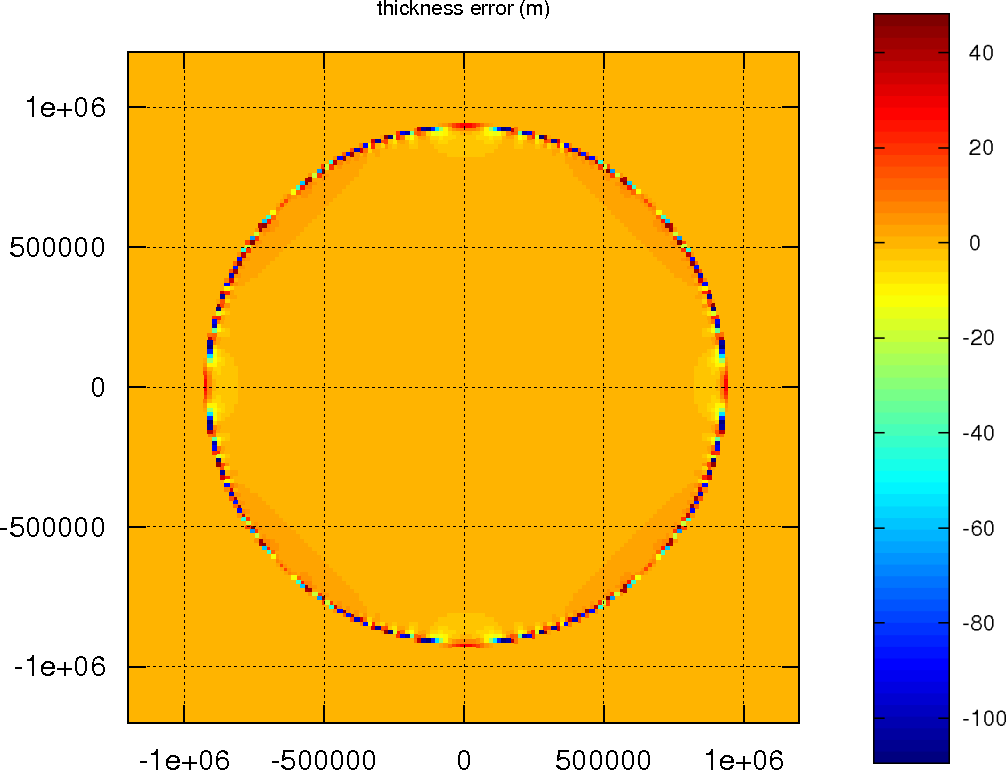
\includegraphics[width=0.7\textwidth]{siaerror}
\end{column}

\begin{column}{0.4\textwidth}
\small
\emph{Trust but verify.}
\medskip

\scriptsize
(Ronald Reagan)

\bigskip\bigskip\bigskip

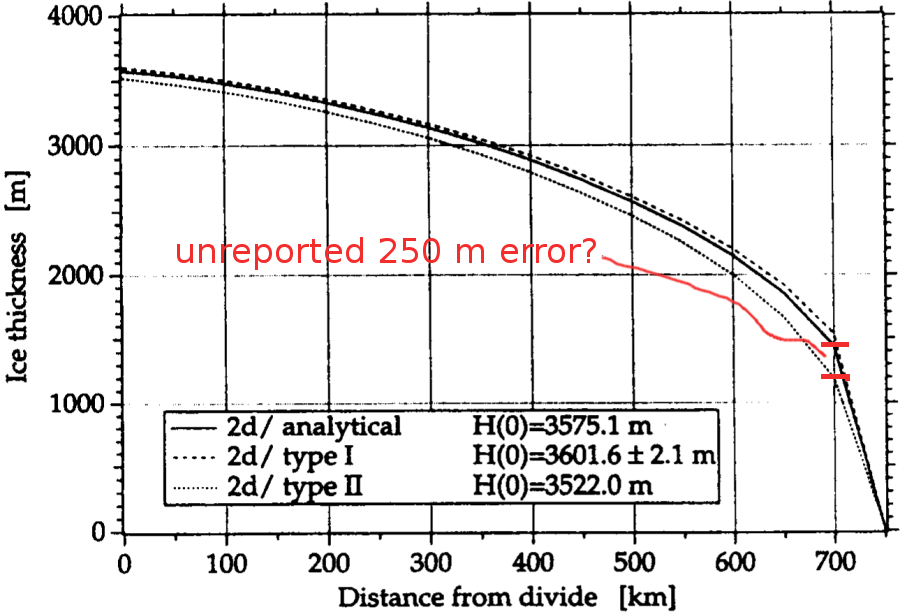
\includegraphics[width=1.0\textwidth]{eismintone}

\scriptsize \emph{figure 2 in Huybrechts et al.~(1996)}
\end{column}
\end{columns}
\end{frame}


\begin{frame}{demonstrate robustness and adaptivity}

\begin{columns}
\begin{column}{0.6\textwidth}
\small
\begin{itemize}
\item test program \texttt{roughice.m} calls \texttt{siaflat.m}
\item sets up the nasty initial state (below left)
\item runs for 50 years
\item get final state (below right)
\item time steps adapt (upper right)
\end{itemize}
\end{column}
\begin{column}{0.4\textwidth}
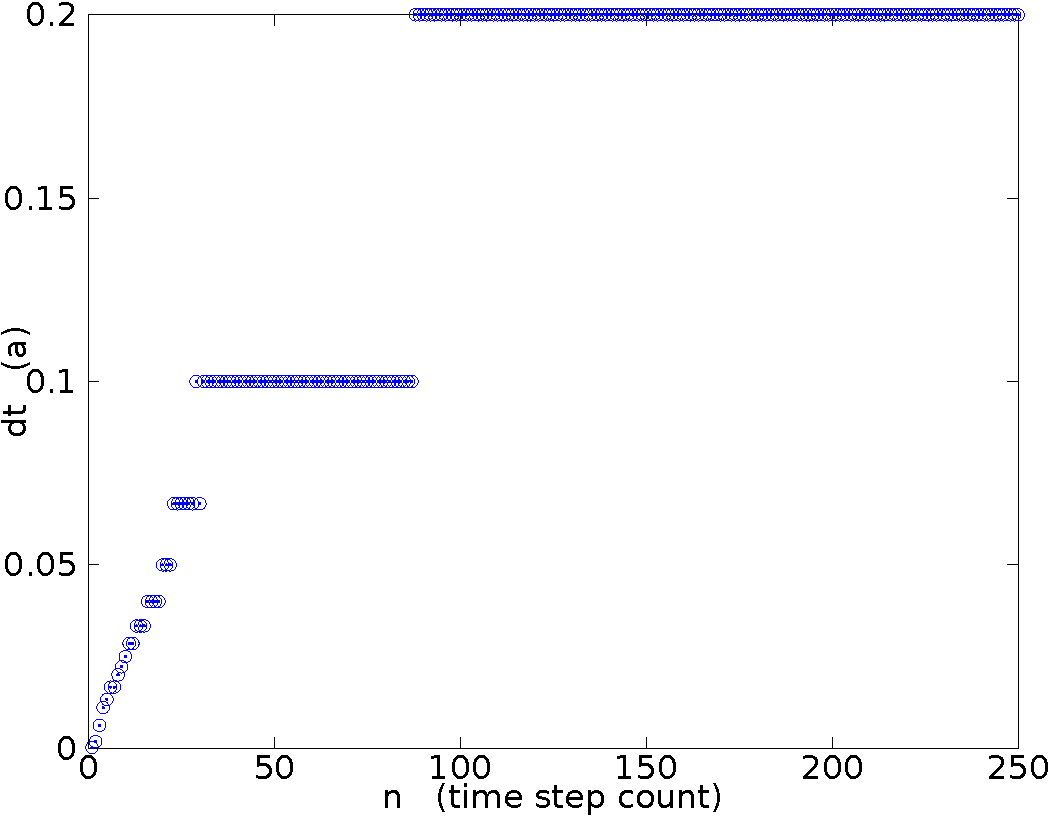
\includegraphics[width=1.0\textwidth]{roughtimesteps}
\end{column}
\end{columns}

\bigskip
\begin{columns}
\begin{column}{0.5\textwidth}
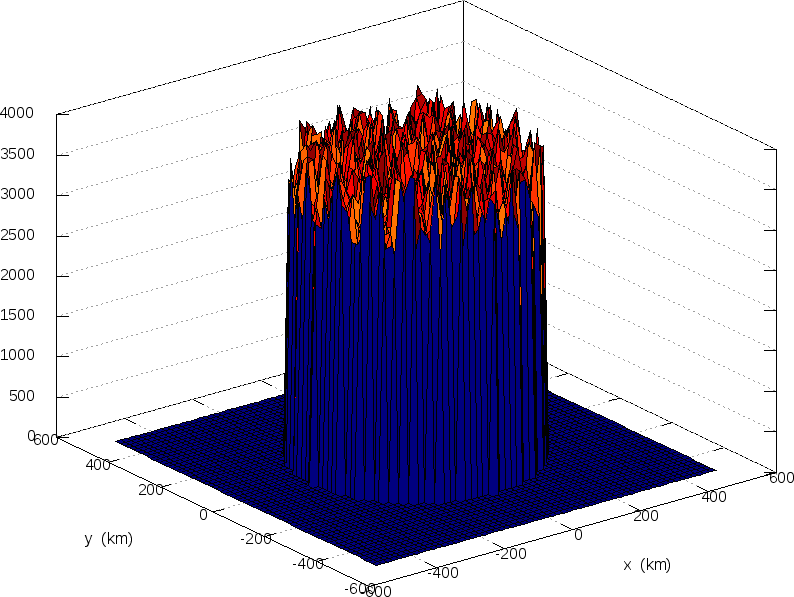
\includegraphics[width=1.0\textwidth]{roughinitial}
\end{column}
\begin{column}{0.5\textwidth}
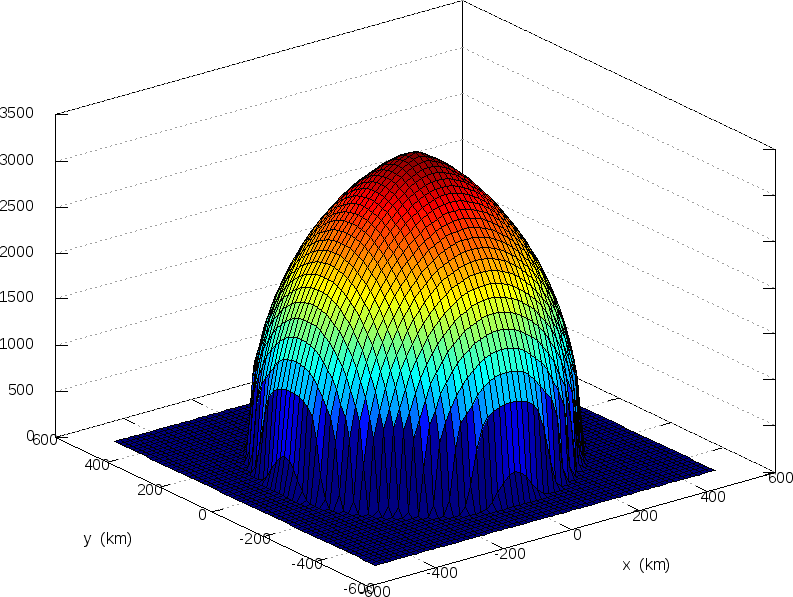
\includegraphics[width=1.0\textwidth]{roughfinal}
\end{column}
\end{columns}
\end{frame}


\begin{frame}{model the Antarctic ice sheet}

\normalsize
\begin{itemize}
\item with careful-but-small modifications of \texttt{siaflat.m}, which make a good exercise:
  \begin{itemize}
  \item[$\circ$] observed accumulation as surface mass balance,
  \item[$\circ$] allow non-flat bed (so $H\ne h$),
  \item[$\circ$] differentiate the surface correctly where floating, and
  \item[$\circ$] calve at current calving front location
  \end{itemize}
here are results from this \emph{toy} Antarctic flow model
\item a 2000 model year run on a $\Delta x=50$ km grid; runtime a few seconds
\end{itemize}

\bigskip

\begin{columns}
\begin{column}{0.4\textwidth}
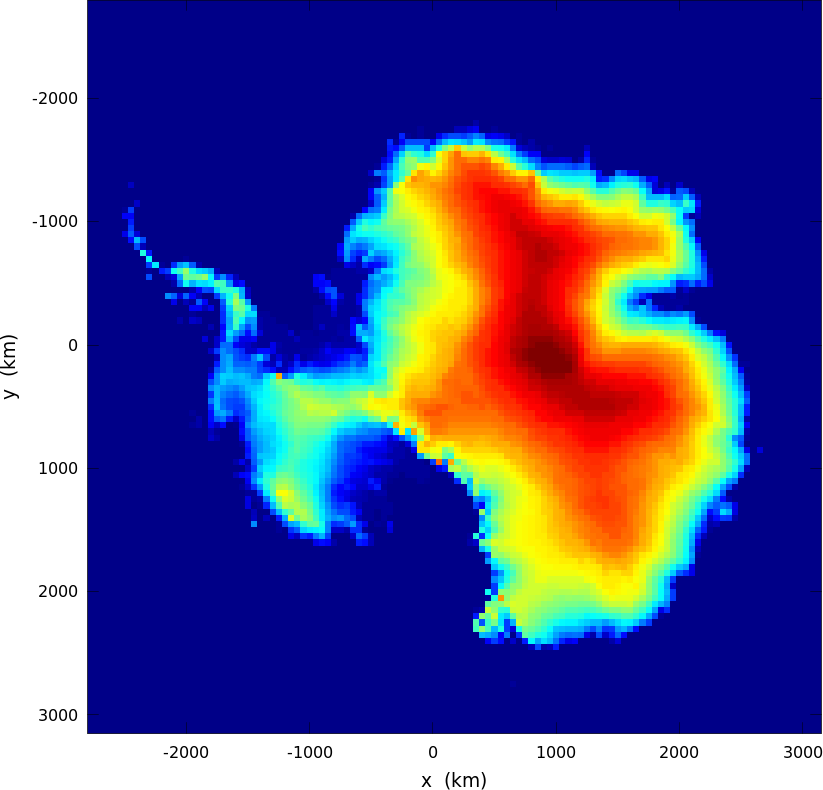
\includegraphics[height=1.75in]{antinitial}
\end{column}
\begin{column}{0.55\textwidth}
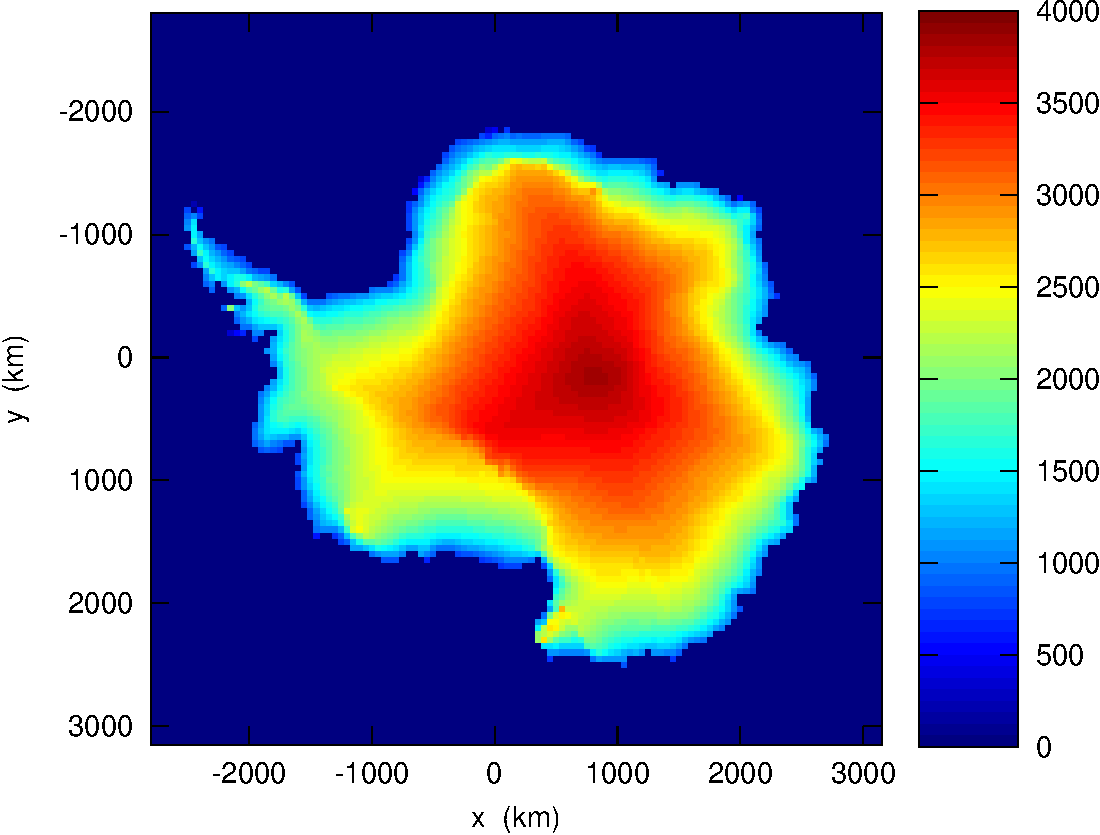
\includegraphics[height=1.75in]{antfinal}
\end{column}
\end{columns}
\end{frame}


\begin{frame}{final comments on SIA: origin and rigor}

where does the ``shallow ice approximation'' come from?:
\bigskip

\begin{itemize}
\item historically, Fowler and Larson (1978), Morland and Johnson (1980), and Hutter (1983) \dots thus recent
\item logically, by a ``small-parameter argument'', based on a small depth-to-width ratio, from the more complete Stokes model for slow ice flow
\item more precisely, by using the small aspect ratio \, $\eps = [H]/[L]$ \, of ice sheets to scale the Stokes model to see which terms make small contributions
\end{itemize}
\end{frame}


\section{shelves and streams}


\subsection{shallow shelf aprx (SSA)}

\begin{frame}{flow model II: shallow shelf approximation (SSA) stress balance}
  
SSA model applies very well to \alert{ice shelves}
\begin{itemize}
\item \dots for parts away from grounding lines
\item \dots and away from calving fronts
\end{itemize}

%\begin{center}
%  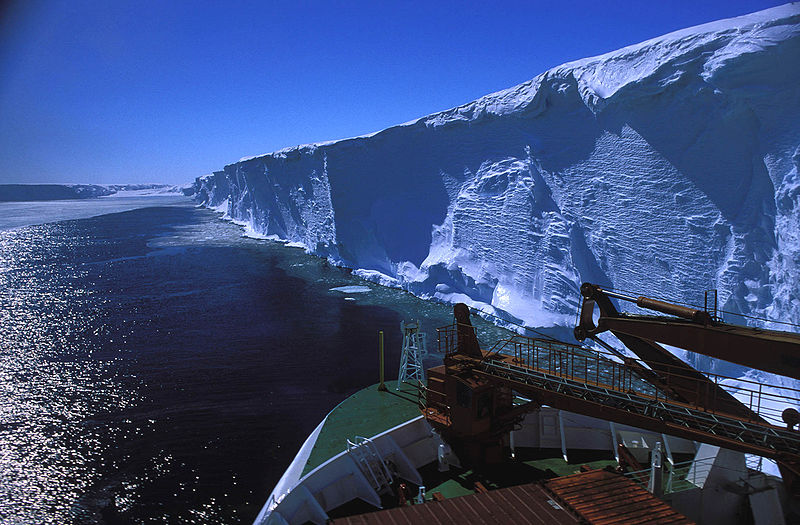
\includegraphics[width=0.7\textwidth]{ice_shelf_edge_hg}
%\tiny edge of Ekstr\"om ice shelf, photo Hans Grobe
%\end{center}
\end{frame}


\begin{frame}{shallow shelf approximation stress balance 2}

SSA also applies reasonably well to \alert{ice streams}
\begin{itemize}
\item \dots with modest bed topography
\item \dots and weak bed strength\footnote{energy conservation (= ice temperature and basal melt) is a major aspect of ice stream flow (Raymond, 2000)\nocite{Raymondenergy}, but not addressed here}
\item imperfect near shear margins and grounding lines
\end{itemize}

\begin{center}
  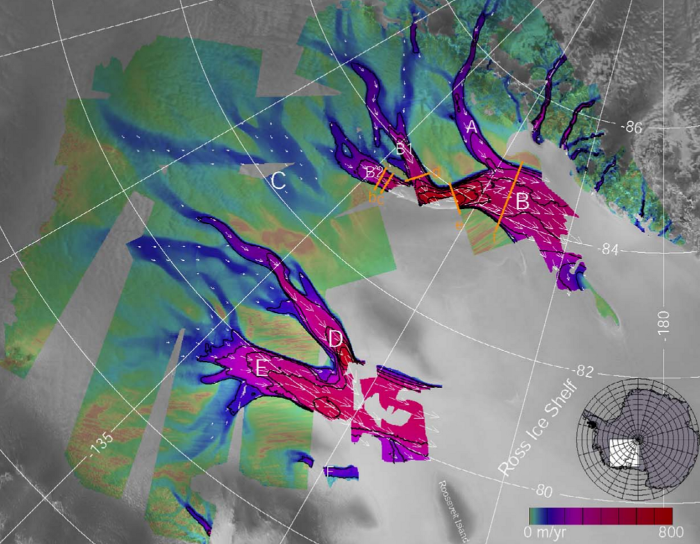
\includegraphics[width=0.6\textwidth]{siple}

\tiny RADARSAT-derived surface velocity for Siple Coast ice streams, Antarctica 
\end{center}
\end{frame}


\begin{frame}{what is, \emph{and is not}, an ice stream?}

\begin{columns}
\begin{column}{0.6\textwidth}
\begin{itemize}
\item ice streams 
  \small
  \begin{itemize}
  \item[$\circ$] slide ($100$ to $1000 \,\text{m}\,\text{a}^{-1}$)
  \item[$\circ$] concentration of vertical shear in a thin layer near base
  \item[$\circ$] \emph{liquid water} at bed plays a critical role (Clarke, 2005)\nocite{Clarke05}
  \end{itemize}
  \normalsize
\item ``outlet glaciers''
  \begin{itemize}
  \item[$\circ$] fast surface speed (up to $10 \,\text{km}\,\text{a}^{-1}$)
  \item[$\circ$] uncertain how much is sliding
  \item[$\circ$] substantial vertical shear ``up'' in the ice column,
  \item[$\circ$] not-at-all flat bed topography
  \item[$\circ$] soft, temperate ice may play a big role
  \end{itemize} 
\item \alert{few simplifying assumptions are appropriate for outlet glaciers}
\end{itemize}
\end{column}

\begin{column}{0.4\textwidth}
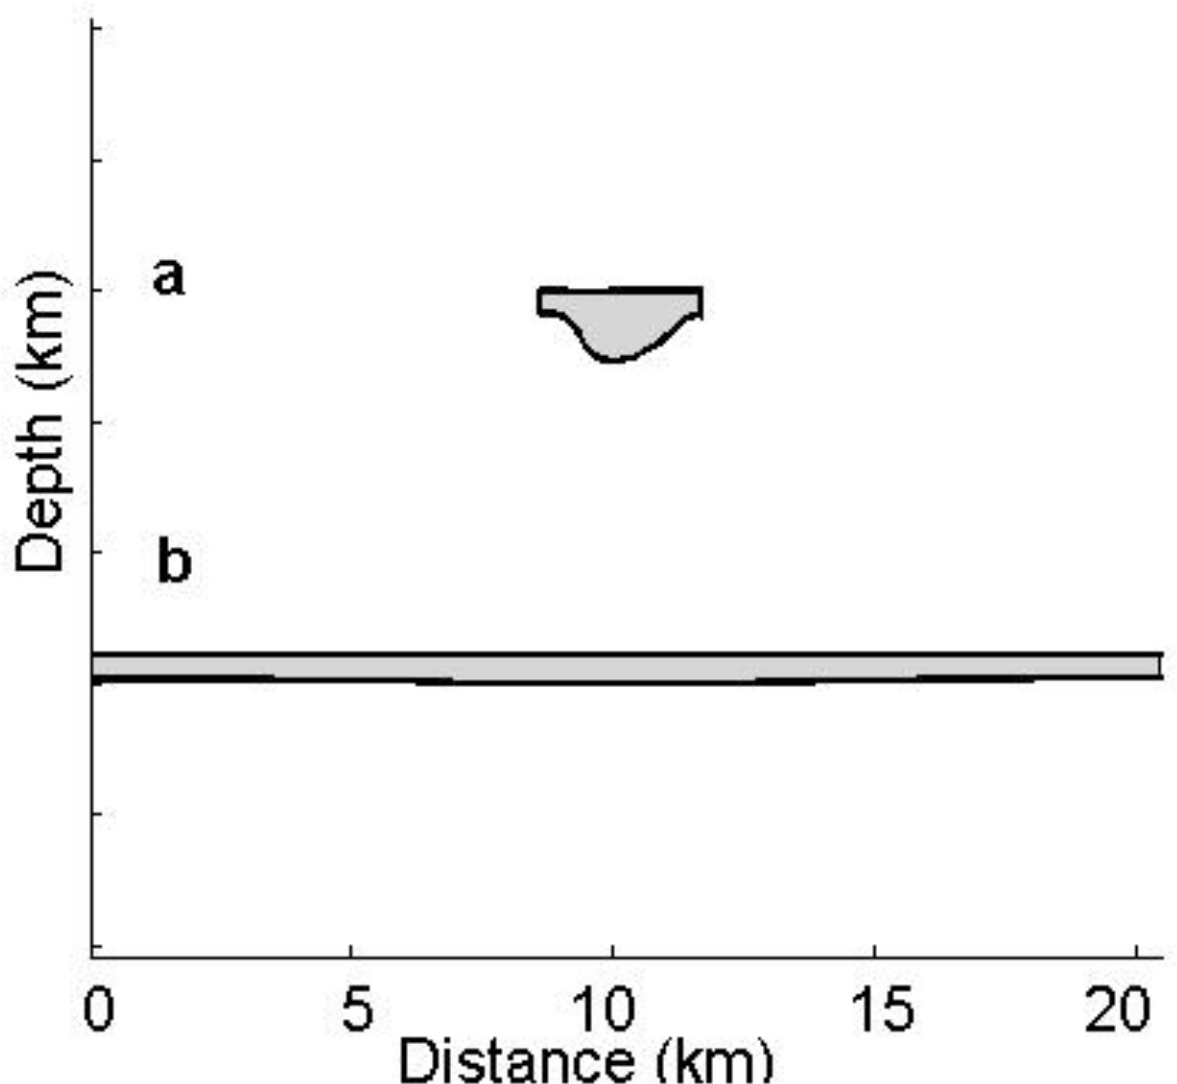
\includegraphics[width=1.0\textwidth]{streamisbrae}

\bigskip
\scriptsize 
Cross sections of Jakobshavns Isbrae (\textbf{a}) and
Whillans Ice Stream (\textbf{b}).  Plotted
without vertical exaggeration.  (\tiny Figure 1 in Truffer and Echelmeyer (2003), \emph{Of isbrae and ice streams}\scriptsize \nocite{TrufferEchelmeyer})
\end{column}
\end{columns}
\end{frame}


\begin{frame}{SSA stress balance equation}

\begin{itemize}
\item only plane flow case (``flow line'')
\item the stress balance equation which determines velocity in an \emph{ice stream}:
\begin{empheq}[box=\fbox]{equation}
  \left({\color{red}2 A^{-1/n} H |u_x|^{1/n - 1} u_x}\right)_x - {\color{blue}C|u|^{m-1}u} = {\color{green}\rho g H h_x} \label{ssa}
\end{empheq}
\item the {\color{red} red term} inside parentheses is the vertically-integrated ``longitudinal'' or ``membrane'' stress
\item the {\color{blue} blue term} is basal resistance
\item the {\color{green} green term} is  driving stress
\item derived originally by Morland (1987)\nocite{Morland}, MacAyeal (1989)\nocite{MacAyeal}
\item \emph{how to think about this equation}?
\item \emph{how do you solve it numerically}?
\end{itemize}
\end{frame}


\begin{frame}{flow line model: from stream to shelf}
\label{slide:streamtoshelf}

\small
\begin{align*}
  u = u_0 & \qquad \text{ at } x = 0 \\
  \left.\begin{array}{r}
  \left(2 A^{-1/n} H |u_x|^{1/n - 1} u_x\right)_x - C|u|^{m-1}u = \rho g H h_x \\
  h = H + b
  \end{array}\right\}& \qquad \text{ on } 0 < x < x_g \\
  \left.\begin{array}{r}
  \left(2 A^{-1/n} H |u_x|^{1/n - 1} u_x\right)_x + 0 = \rho g H h_x \\
  h = (1-\rho/\rho_w) H
  \end{array}\right\}& \qquad \text{ on } x_g < x < x_c \\
  2 A^{-1/n} H |u_x|^{1/n - 1} u_x = \frac{1}{2}\rho (1-\rho/\rho_w) g H^2 & \qquad \text{ at } x = x_c
\end{align*}

\bigskip\bigskip
\begin{center}
  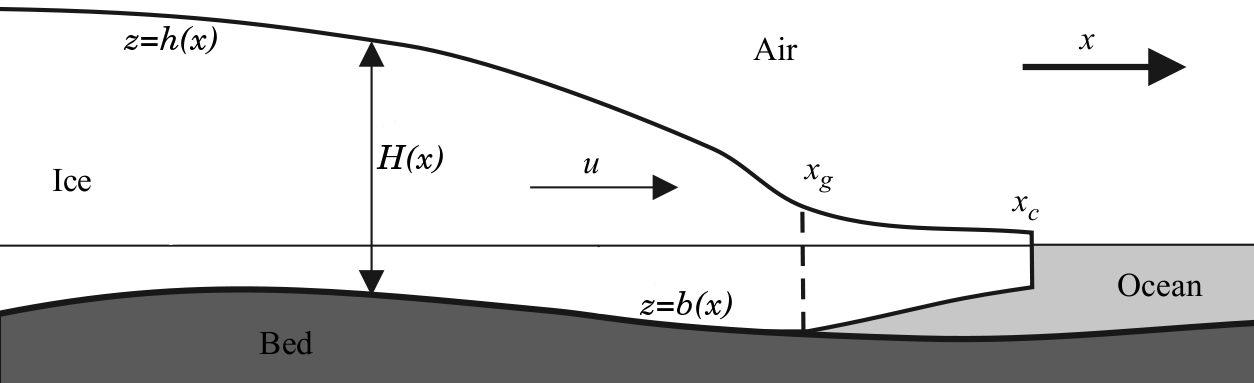
\includegraphics[width=0.7\textwidth]{flowline}
\end{center}
\end{frame}


\begin{frame}{flotation criterion and grounding line}

\begin{itemize}
\item the inequality ``$\rho H < - \rho_w b$'' is the \alert{flotation criterion}
\item at the grounding line $x=x_g$ the above inequality switches
\item \dots and the driving stress switches form:
  \begin{itemize}
  \item[$\circ$] on the grounded side we know $\rho H > - \rho_w b$ so
  	$$\rho g H h_x = \rho g H (H_x + b_x)$$
  \item[$\circ$] on the floating side we know $\rho H < - \rho_w b$ so $h = (1-\rho/\rho_w) H$ and so
  	$$\rho g H h_x = \rho(1-\rho/\rho_w) g H H_x$$
  \end{itemize}
\item also: $H,u,u_x$ are all continuous at $x=x_g$
\item best numerical models for moving grounding lines still an open question (e.g.~MISMIP and all that)
\end{itemize}
\end{frame}



\subsection{ice shelf flow line solution}


\begin{frame}{exact velocity and thickness for steady ice shelf}

\begin{itemize}
\item limited goal here: describe a steady state, 1D ice shelf
\item there is this nice \alert{by-hand} result (next slide): the thickness and velocity in the ice shelf can be completely determined \nocite{MacAyealBarcilon,vanderVeen85} in terms of the 
  \begin{enumerate}
  \item ice thickness $H_g$ at the grounding line and
  \item ice velocity $u_g$ at the grounding line
  \end{enumerate}
\item we will use this to
  \begin{itemize}
  \item[$\circ$] understand the SSA better
  \item[$\circ$] verify a numerical SSA code
  \end{itemize}
\end{itemize}
\end{frame}


\begin{frame}{exact velocity and thickness for steady ice shelf 2}

\small see \texttt{testshelf.m} 

\begin{center}
  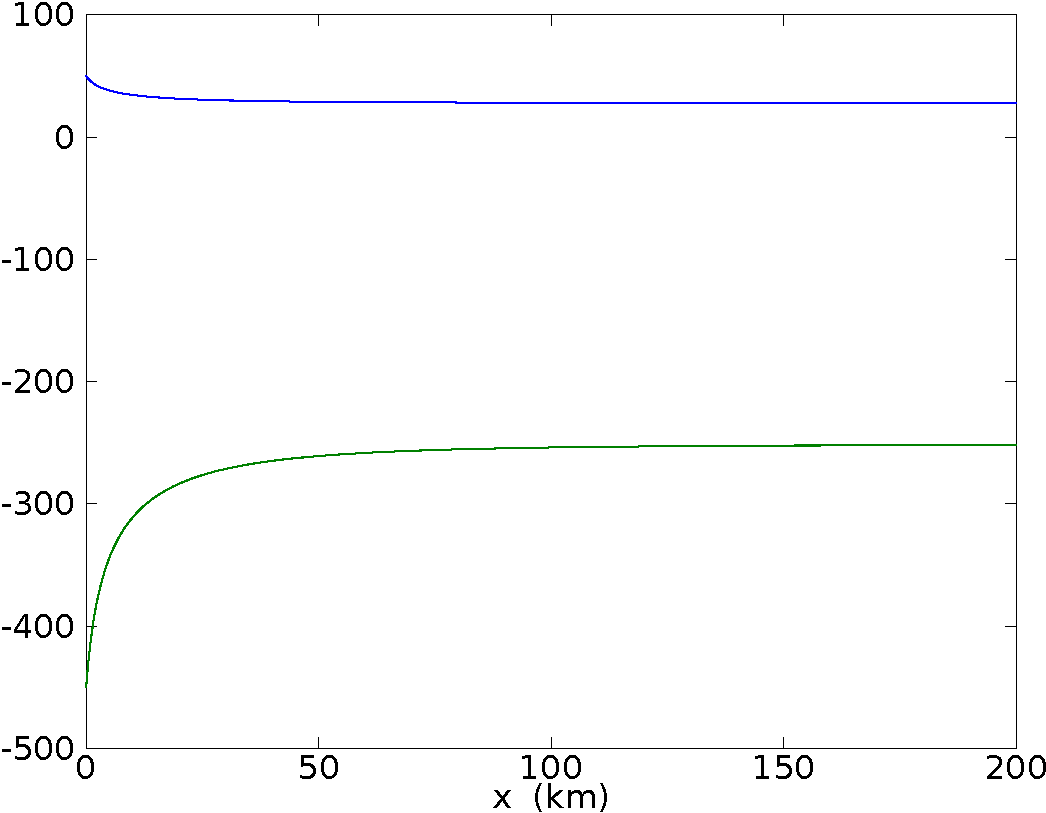
\includegraphics[width=0.45\textwidth]{steadyshelfprofile} \quad
  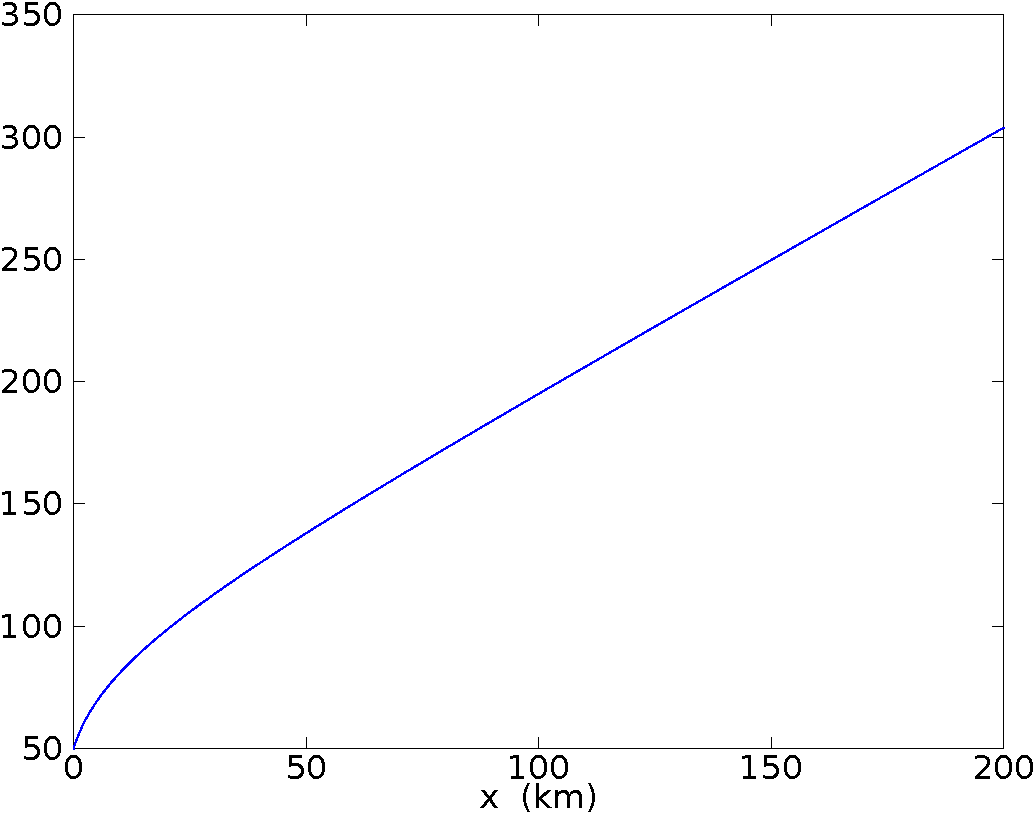
\includegraphics[width=0.45\textwidth]{steadyshelfvelocity}
\end{center}

\bigskip\bigskip
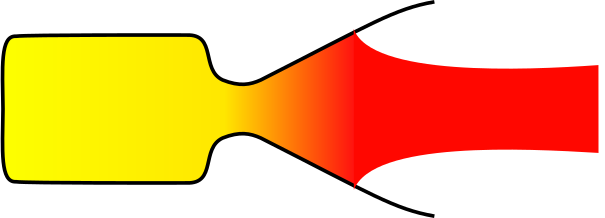
\includegraphics[width=0.3\textwidth]{Rocket_nozzle_expansion}
\end{frame}


\subsection{numerical SSA}

\begin{frame}{numerically solving the SSA stress balance}

\begin{itemize}
\item here we fix ice thickness $H(x)$ and find the velocity numerically
\item the stress balance is a nonlinear equation in the velocity:
  $$\left(2 A^{-1/n} H |u_x|^{1/n - 1} u_x\right)_x - C|u|^{m-1}u = \rho g H h_x$$
\item \alert{iteration is needed}
\item I'll describe the numerical method for a shelf \emph{or} stream, but only give a code for an ice shelf
\end{itemize}
\end{frame}


\begin{frame}{numerically solving the SSA stress balance 2}

\begin{itemize}
\item coefficient ${\color{red} \bar \nu} = A^{-1/n} |u_x|^{1/n-1}$ is the ``effective viscosity'':
   $$\left(2 \,{\color{red} \bar \nu}\, H u_x\right)_x - C |u|^{m-1} u = \rho g H h_x$$
\item \emph{simplest iteration idea}: use old effective viscosity to get new velocity solution, and repeat until things stop changing
  \begin{itemize}
  \item[$\circ$] this is ``Picard'' iteration
  \item[$\circ$] Newton iteration is a superior alternative
  \end{itemize}
\item specifically:
  \begin{itemize}
  \item[$\circ$] last iterate $u^{(k-1)}$
  \item[$\circ$] define $W^{(k-1)} = 2 \bar \nu H = 2 A^{-1/n} |u^{(k-1)}_x|^{1/n-1} H$
  \item[$\circ$] current iterate (unknown) $u^{(k)}$
  \item[$\circ$] solve repeatedly:
     $$\left(W^{(k-1)} u^{(k)}_x\right)_x - C |u^{(k-1)}|^{m-1} u^{(k)} = \rho g H h_x$$
  \end{itemize}
\end{itemize}
\end{frame}


\begin{frame}{solving the ``inner'' linear problem}
\begin{itemize}
\item abstract the problem:
   $$\left(W(x)\, u_x\right)_x - \alpha(x)\, u = \beta(x)$$
on $0 < x < L$, with boundary conditions
   $$u(0) = V, \qquad  u_x(L) = \gamma$$
\item an \emph{elliptic} PDE boundary value problem
\item $W(x)$, $\alpha(x)$, $\beta(x)$ are known functions in the SSA context:
  \begin{itemize}
  \item[$\circ$] both $W(x)$ and $\alpha(x)$ come from previous iteration
  \item[$\circ$] $\beta(x)$ is driving stress
  \end{itemize}
\end{itemize}
\end{frame}


\begin{frame}{where do you get an initial guess $u^{(0)}$?}

\begin{itemize}
\item \emph{for floating ice}, a possible initial guess for velocity comes from assuming a uniform strain rate:
   $$u^{(0)}(x) = \gamma (x-x_g) + u_g$$
where $\gamma$ is the value of $u_x$ found from calving front stress imbalance
\item \emph{for grounded ice}, a possible initial guess for velocity is to assume ice is held by basal resistance only:
   $$u^{(0)}(x) = \left(-C^{-1} \rho g H h_x\right)^{1/m}$$
\end{itemize}
\end{frame}


\begin{frame}{numerics of the ``inner'' linear problem}

\begin{itemize}
\item suppose $j=1,2,\dots,J+1$, where $x_1 = x_g$ and $x_{J+1} = x_c$ are endpoints
\item $W(x)$ is needed on the staggered grid; the approximation is:
$$\frac{W_{j+1/2} (u_{j+1} - u_j) - W_{j-1/2} (u_{j} - u_{j-1})}{\Delta x^2} - \alpha_j u_j \stackrel{\ast}{=} \beta_j$$
\item left-hand boundary condition: $u_1 = V$ given
\item right-hand boundary condition (``$u_x(L)=\gamma$''):
  \begin{itemize}
  \item[$\circ$] introduce notional point $x_{J+2}$
  \item[$\circ$]
    $$\frac{u_{J+2} - u_J}{2 \Delta x} = \gamma$$
  \item[$\circ$] using equation $\ast$ in $j=J+1$ case, eliminate $u_{J+2}$ variable ``by-hand'' before coding numerics \nocite{MortonMayers}
  \end{itemize}
\end{itemize}
\end{frame}


\begin{frame}{numerics of the ``inner'' linear problem 2}

\scriptsize
\begin{itemize}
\item so SSA stress balance has form  \quad $A \mathbf{x} = \mathbf{b}$, \quad namely:
$$
\begin{bmatrix}
1 &  &  &  &  \\
W_{3/2} & A_{22} & W_{5/2} &  &  \\
 & W_{5/2} & A_{33} &  &  \\
 &  & \ddots & \ddots &  \\
 &  & W_{J-1/2} & A_{JJ} & W_{J+1/2} \\
 &  &  & A_{J+1,J} & A_{J+1,J+1} \\
\end{bmatrix}\,
\begin{bmatrix}
u_1 \\ u_2 \\ u_3 \\ \vdots \\ u_J \\ u_{J+1}
\end{bmatrix}
=
\begin{bmatrix}
0 \\ \beta_2 \Delta x^2 \\ \beta_3 \Delta x^2 \\ \vdots \\ \beta_J \Delta x^2 \\ b_{J+1}
\end{bmatrix}
$$
\item with diagonal entries
$$A_{22} = -(W_{3/2}+W_{5/2}+\alpha_1 \Delta x^2)$$
$$A_{33} = -(W_{5/2}+W_{7/2}+\alpha_2 \Delta x^2)$$
and so on, up to $A_{JJ}$, 
\item with special cases in last equation:
$$A_{J+1,J} = 2 W_{J+1/2}$$
$$A_{J+1,J+1} = -(2 W_{J+1/2}+\alpha_{J+1}\Delta x^2)$$
$$b_{J+1} = -2 \gamma \Delta x W_{J+3/2} + \beta_{J+1} \Delta x^2$$
\item this is a \emph{tridiagonal} system
\end{itemize}
\end{frame}


\begin{frame}{numerics of the ``inner'' linear problem 3}
\label{slide:flowlinecode}

\minput{flowline}
\end{frame}


\begin{frame}{testing the ``inner'' linear code}

\begin{itemize}
\item before proceeding to solve nonlinear SSA problem, we can test the ``abstracted'' code \texttt{flowline.m}
\item test by ``manufacturing'' solutions
  \begin{itemize}
  \item[$\circ$] see \texttt{testflowline.m}; not shown
  \end{itemize}
\item results:
  \begin{itemize}
  \item[$\circ$] converges at optimal rate $O(\Delta x^2)$
  \end{itemize}
\end{itemize}
\end{frame}


\begin{frame}{numerical: SSA}

\minputtiny{ssaflowline}
\end{frame}


\begin{frame}[fragile]
  \frametitle{\emph{numerical} thickness and velocity for steady ice shelf}

lines below are a convergence analysis of \texttt{testshelf.m}, which calls \texttt{ssaflowline.m}:

\begin{center}
  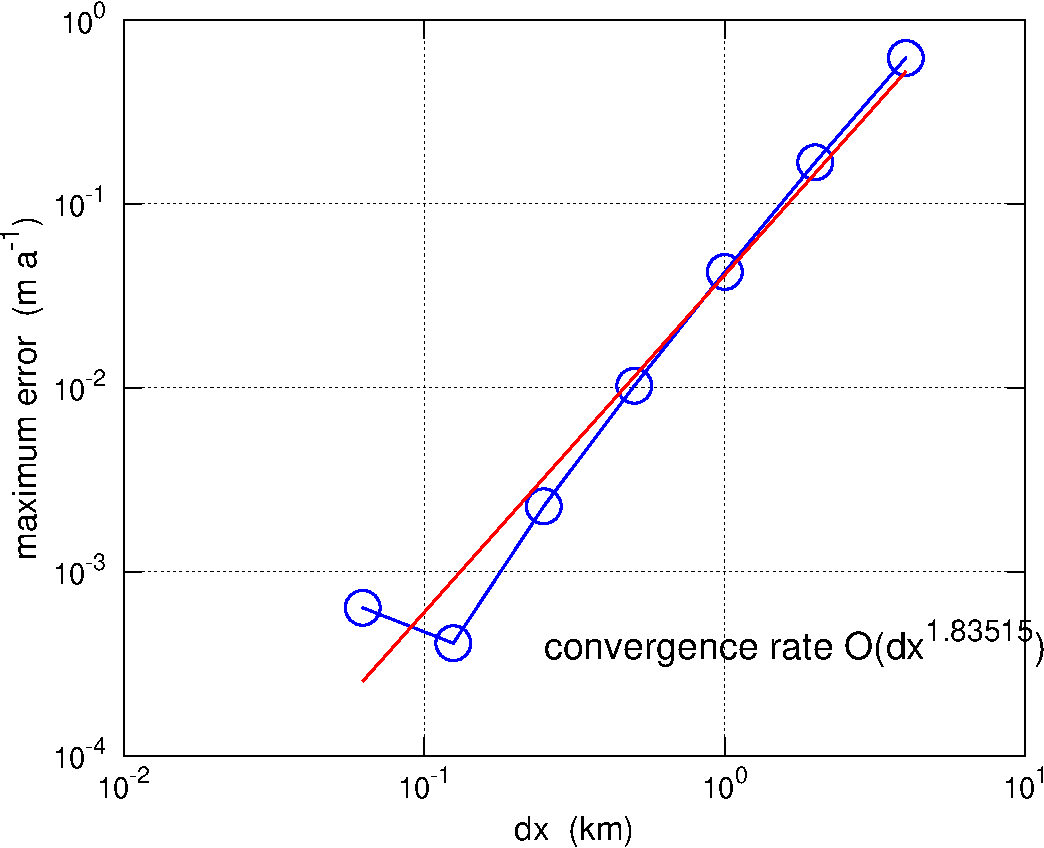
\includegraphics[width=0.75\textwidth]{shelfconv}
\end{center}
\end{frame}


\begin{frame}{SSA model output}

\begin{center}
  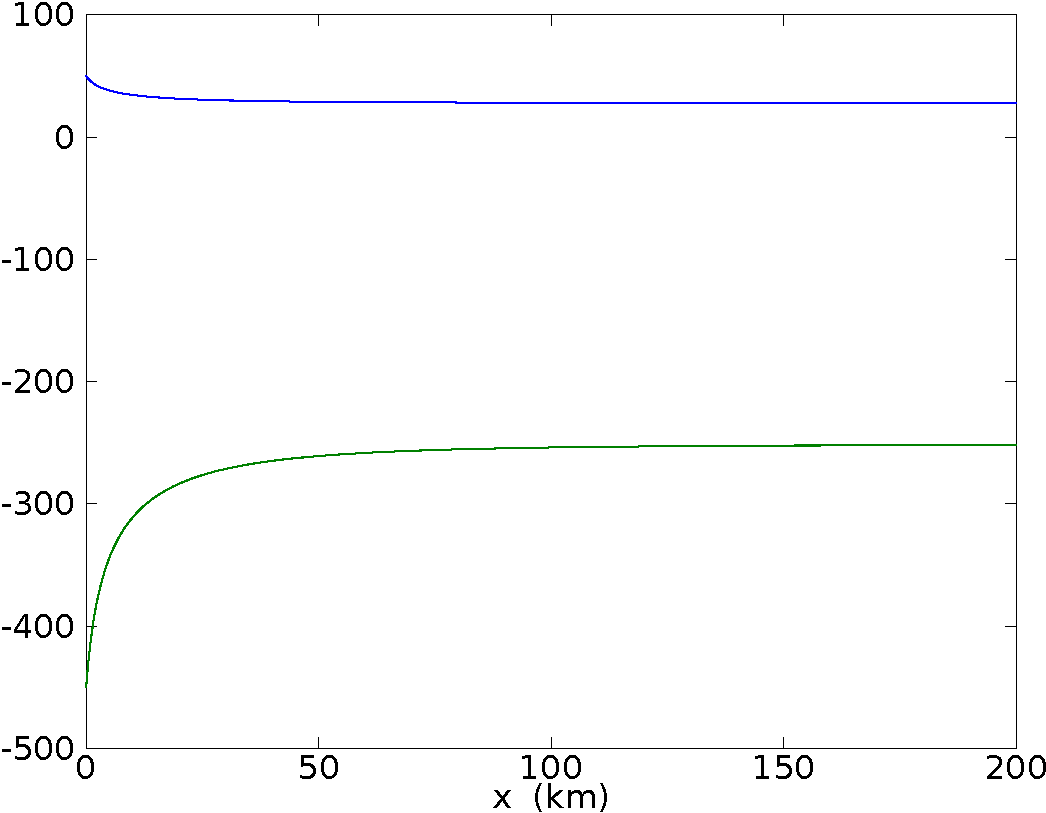
\includegraphics[width=0.45\textwidth]{steadyshelfprofile} \quad
  \includegraphics[width=0.45\textwidth]{steadyshelfvelocity}
\end{center}

\bigskip

\begin{itemize}
\item \emph{this looks suspiciously like figures for the exact solution \dots}
\item yes
\end{itemize}
\end{frame}


\begin{frame}{realistic ice shelf modeling}

\begin{itemize}
\item flow lines are never very realistic
\item you can add parameterized ``side drag'' \dots
\item also, ice shelves have surprises:
  \begin{itemize}
  \item[$\circ$] high basal melt near grounding lines
  \item[$\circ$] marine ice can freeze-on at bottom (below)
  \item[$\circ$] ``reverse slope'' bed instability and WAIS \dots
  \end{itemize}
\end{itemize}

\medskip
\begin{center}
  \includegraphics[width=0.5\textwidth]{marineice}
  
  \medskip
  \tiny from Grosfeld \& Thyssen 1994 \nocite{GrosfeldThyssen1994}
\end{center}
\end{frame}


\begin{frame}{ice shelf modeling in 2D}

\begin{itemize}
\item nonetheless ``diagnostic'' (static geometry) ice shelf modeling in 2d has been quite successful
\item observed surface velocities validate SSA stress balance model
  \begin{itemize}
  \item[$\circ$] e.g.~Ross ice shelf example below using PISM
  \item[$\circ$] \dots but many models can do this
  \end{itemize}
\end{itemize}

\begin{center}
  \includegraphics[width=0.5\textwidth]{rossquiver} \quad  \includegraphics[width=0.45\textwidth]{rossscatter}
\end{center}
\end{frame}


\begin{frame}{numerical solution of stress balances: a summary}

\begin{itemize}
\item stress balance equations (e.g.~SSA or Stokes) determine velocity from geometry and boundary conditions
  \begin{itemize}
  \item[$\circ$] nonlinear so iteration is necessary
  \item[$\circ$] at each iteration a sparse matrix ``inner'' problem is solved \dots give it to a matrix solver software package
  \end{itemize}

\bigskip
\item general principles:
  \begin{itemize}
  \item[$\circ$] \alert{modularize your code}
  \item[$\circ$] \alert{test the parts}
  \end{itemize}
\end{itemize}
\end{frame}


\begin{frame}{the mass continuity equation: a summary}

\begin{itemize}
\item the \emph{mass continuity equation} is
  $$H_t = M - \nabla \cdot (\mathbf{u} H)$$
\item the numerical nature of this equation depends on the stress balance:
  \begin{itemize}
  \item[$\circ$] the equation is a diffusion for frozen bed, large scale flows (i.e.~SIA)
  \item[$\circ$] it is \emph{not} very diffusive for membrane stresses and no basal resistance (e.g.~SSA for ice shelves)
  \item[$\circ$] it is diffusive for ice streams (but how much?)
  \item[$\circ$] there is \emph{not} much helpful theory on this transport problem
  \item[$\circ$] \dots maybe you will help find this theory!
  \end{itemize}
\end{itemize}
\end{frame}



% Copyright 2009--2010  Ed Bueler

\section{next steps}

\subsection{practicalities}

\begin{frame}[fragile]
\frametitle{what technical skills are needed for \\ numerical ice sheet modeling?}

you need:

\begin{itemize}
\item comfort in a technical computing environment, usually Unix, in which you need to know:
  \begin{itemize}\small
  \item[$\circ$] an editor,
  \item[$\circ$] a compiled language (Fortran or C),
  \item[$\circ$] a scripting/prototyping language (Matlab, Python, etc.), and
  \item[$\circ$] \emph{a version control system} (Subversion, git, etc.)
  \normalsize
  \end{itemize}
\item willingness to read math, numerical analysis, computer science books
\item \dots and willingness to ignor \emph{some} of the advice found there
\item know some tools for NetCDF files
\item get exposed to parallel computing
\item but, at the end of the day: \emph{physics}
\end{itemize}
\end{frame}


\begin{frame}
\frametitle{what technical skills are needed? 2}

\begin{itemize}
\item an important skill is to \emph{not} re-invent the wheel
\item \emph{never} re-invent the wheel for basic numerics:
  \begin{itemize}
  \item[$\circ$] \Matlab, Comsol, PETSc, libmesh, Elmer, Trilinos, Triangle, etc.~handle fundamental numerical linear algebra, mesh generation, finite element assembly and solve, etc.~tasks; don't even try to compete!
  \item[$\circ$] \dots except to write throw-away codes to help you \emph{understand} numerical ideas 
  \end{itemize}
\item sometimes there is no need to re-invent ice sheet modeling:
  \begin{itemize}
  \item[$\circ$] open source SIA-based comprehensive models: GLIMMER, SICOPOLIS
  \item[$\circ$] open source hybrid/higher-order/Stokes models: PISM, Elmer-ice, CISM
  \end{itemize}
\item glacier and ice sheet modeling is young!  there is much to do!
\end{itemize}
\end{frame}


\subsection{omitted models}

\begin{frame}{omitted models 1: thermomechanical coupling}

\begin{columns}
\begin{column}{0.6\textwidth}
\begin{itemize}
\item the softness of ice ``$A$'' is not constant!
  \begin{itemize}
  \item[$\circ$] $A=A(T)$ varies by more than $10^3$ in the $50\phantom{|}^\circ\text{C}$ ice temperature range relevant to Antarctic ice
  \item[$\circ$] dissipation of flow energy is significant in conservation of energy equation
  \item[$\circ$] \dots and there is a ``new'' fluid instability from feedback between the above two items \scriptsize (lower figure; EISMINT II [Payne and others, 2000]\nocite{EISMINT00}) \small
  \end{itemize}
\item ice temperature is part of the ``long memory'' of the ice sheets for past climate
\item conservation of energy is just as important for fast scale dynamics (involving sliding and hydrology) as it is for ``long memory'' questions
\end{itemize}
\end{column}
\begin{column}{0.4\textwidth}
\vspace{-0.2in}
  \includegraphics[width=1.0\textwidth]{pdffigs/AofT}
  
\bigskip
  \includegraphics[width=1.0\textwidth]{photos/eisIIF}
\end{column}
\end{columns}
\end{frame}


\begin{frame}{omitted models 2: surface mass balance}

\begin{itemize}
\item ice sheet models need \emph{modeled} surface mass balance
  \begin{itemize}
  \item[$\circ$] over paleoglacial time scales
  \item[$\circ$] and when modeling response to future changes
  \end{itemize}
\item models include:
  \begin{itemize}
  \item[$\circ$] positive degree-day (PDD) and other index models
  \item[$\circ$] energy-balance models
  \end{itemize}
\nocite{Hock05}
%\item read: [Hock, 2005]\nocite{Hock05} $=$ survey of observations and processes
\item very significant source of uncertainty for Greenland ice sheet dynamics!
\end{itemize}
\end{frame}


\begin{frame}{omitted models 3: solid Earth deformation}

\begin{itemize}
\item ice has almost $\frac{1}{3}$ of the density of the viscous hot rock in the Earth's mantle,
\item so 1000 m of ice will depress the Earth's crust almost 300 m if allowed enough time
\item this changes bed topography and thus ice flow, so Earth deformation is important to modeling ice flow
\item read?:
  \begin{itemize}
  \item[$\circ$] [Peltier, 1998]\nocite{Peltier1998review} $=$ survey of observations and processes
  \item[$\circ$] [Greve, 2001]\nocite{Greve2001} $=$ comparison of practical models
  \end{itemize} 
\end{itemize}

\begin{center}
  \includegraphics[width=0.75\textwidth]{photos/earthcompare}
\end{center}
\end{frame}


\begin{frame}{omitted models 4: numerical Stokes equations}

\begin{itemize}
\item the Stokes model itselfcan be solved numerically
  \begin{itemize}
  \item[$\circ$] no shallow assumptions!
  \item[$\circ$] but many more equations and unknowns than SIA, SSA, hybrids, Blatter, \dots
  \end{itemize}
\item requires \emph{explicit} accounting for
  \begin{itemize}
  \item[$\circ$] incompressibility $=$ a constraint on the flow
  \item[$\circ$] pressure $=$ a Lagrange multiplier for that constraint
  \end{itemize} 
\item very tough scalability issues:  can you afford the loss of resolution?  loss of long-time runs?
\item all of the success so far is at a smaller scale (e.g.~below)
\end{itemize}

\begin{columns}
\begin{column}{0.45\textwidth}
\scriptsize
Figure 7 in [Maxwell and others, 2008]\nocite{Maxwelletal2008}: \emph{Athabasca Glacier:  (a) modeled velocity contour lines ($\text{m}\,\text{a}^{-1}$); (b) contour lines derived from measurements [Raymond, 1971]\nocite{Raymond1971}}
\end{column}
\begin{column}{0.6\textwidth}
\includegraphics[width=0.75\textwidth]{photos/athabasca_cross}
\end{column}
\end{columns}
\end{frame}


\begin{frame}{omitted models 5: ``higher-order'' schemes}

\begin{itemize}
\item both the SIA and the SSA are derived by small-parameter arguments from the Stokes equations, so \dots
\item is there a \emph{common shallow antecedent model}?
\item Schoof and Hindmarsh [2009]\nocite{SchoofHindmarsh} answer:
  \begin{itemize}
  \item[$\circ$] \emph{yes}, the Blatter [1995]\nocite{Blatter} model is  intermediate between the Stokes stress balance and both the SIA and SSA
  \end{itemize}
\end{itemize}

\begin{center}
\includegraphics[width=0.7\textwidth]{photos/hierarchy}
\end{center}
\end{frame}



\begin{comment}
REMEMBER TO THINK ABOUT THESE THINGS:
* SSA numerics use matrix solution: point out general sparseness and methods?  exercise related to methods?
* attempt to use Green's function to understand diffusivity of 1D SSA?
* why is ice sheet modeling a "1 bar subject"?
* ED: make sure to test codes in Matlab
* add slide for SIA: "careful with the smoothness of the bed ... because you are differentiating it"   show equation   H_t = M + \Div (D \grad H) + \Div(D \grad b)
* Walt-style props
   -- bicycle for plastic till analogy
   -- membrane and grid for free boundary
   -- silly putty
\end{comment}


% extra slides on free-boundary problems:
%   put these in when building refs
%   put these in for actual lecture
%   do not put these in when printing out
% Copyright 2009--2012  Ed Bueler

%\section{free boundary problems}

\begin{frame}{\emph{POSTSCRIPT} on free boundary value problems}

\begin{itemize}
\item ice sheet/shelf modeling means free boundary problems
\item Hutter [1999] identifies some below
\end{itemize}
\begin{center}
  \includegraphics[width=0.8\textwidth]{photos/freehutter}
\end{center}
\end{frame}


\begin{frame}{what is a ``free boundary''?}

\begin{itemize}
\item a \emph{free boundary} for a PDE is an unknown location at which there is a boundary condition
  \begin{itemize}
  \item[$\circ$] the location of the free boundary must be found at the same time as one solves the PDE problem
  \item[$\circ$] in addition to the information which would already be present at a fixed-location boundary, there must be enough additional information at a free boundary to determine its location
  \item[$\circ$] all free boundary problems are nonlinear, regardless of the linearity of the PDE
  \end{itemize}
\item classic \emph{example}:  consider an elastic membrane attached to a wire frame and stretched over an obstacle:
\end{itemize}

\begin{columns}
\begin{column}{0.5\textwidth}
\small
constraint:
  $$u \ge \psi$$

in locations where $u>\psi$, solve:
  $$\grad^2 u = 0$$
  
\emph{where is the free boundary, and what facts about $u$ are true there?}
\end{column}
\begin{column}{0.5\textwidth}
  \includegraphics[width=1.0\textwidth]{photos/classicalobs}
\end{column}
\end{columns}
\end{frame}


\begin{frame}{free boundary value problem 1: polythermal ice}

\small
\begin{itemize}
\item by volume, majority of ice sheet is \emph{cold} ($T < 0\phantom{|}^\circ\text{C}$)
\item \dots but there is some ice which is \emph{temperate}, where $T = 0\phantom{|}^\circ\text{C}$ \emph{and} there is a positive liquid fraction within the ice matrix
\item \dots so ice sheets are \emph{polythermal}
\item boundary between cold and temperate ice is ``CTS'' (= cold-temperate transition surface):
  \begin{itemize}
  \item[$\circ$] must be found, as free boundary, when solving conservation of energy equation (``Stefan problem'')
  \item[$\circ$] can be tracked explicitly [Greve, 1997]
  \item[$\circ$] or treated as a level surface of the enthalpy variable [Aschwanden et al, 2012]
  \end{itemize}
%\item \emph{side note}: for temperate ice there must be some dependence of ice strength (e.g.~softness $A$ in Glen law), but only one reference we can find [Lliboutry and Duval, 1985]
\end{itemize}

\begin{center}
\includegraphics[width=0.8\textwidth]{photos/polythermal_types}
\end{center}
\end{frame}


\begin{frame}{free boundary value problem 2: for ice streaming}

%\vspace{-0.2in}
\begin{itemize}
\item  Schoof's [2006] insight, for diagnostic case
  $$\text{SSA + (plastic till)} = \begin{pmatrix}
\text{well-posed free boundary problem} \\ \text{for location \emph{and} velocity of sliding}
\end{pmatrix} $$
\item ``plastic till'' means the basal strength (resistance) is given by a yield stress $\tau_c$:  \qquad $\vec\tau_b = \tau_c \mathbf{v}_b / |\mathbf{v}_b|$
\item Schoof's scheme is a \emph{whole ice sheet form} of MacAyeal's [1989] individual ice stream models
\end{itemize}

\begin{columns}
\begin{column}{0.5\textwidth}
\begin{center}
  \includegraphics[width=1.0\textwidth]{photos/schoof_planform}
\end{center}
\end{column}
\begin{column}{0.5\textwidth}
\begin{center}
  \includegraphics[width=0.95\textwidth]{photos/schoof_sliders}
\end{center}
\end{column}
\end{columns}
\end{frame}


\begin{frame}{free boundary problem 3: for grounded ice sheet margin}

\begin{itemize}
\item side-by-side comparison, \emph{classical elastic membrane problem} versus \emph{steady ice sheet problem}
\end{itemize}
\small
\begin{columns}[T]
\begin{column}{0.4\textwidth}
constraint:
  $$u \ge \psi$$

where $u>\psi$, solve:
  $$\grad^2 u = 0$$

\bigskip
\includegraphics[width=0.8\textwidth]{photos/classicalobs}
\end{column}
\begin{column}{0.6\textwidth}
constraint:
  $$h \ge b \qquad \iff \qquad H \ge 0$$

where $h>b$, solve steady SIA:
  $$0 = M + \Div \left(\Gamma H^{n+2} |\grad h|^{n-1} \grad h \right)$$

\bigskip
\includegraphics[width=0.9\textwidth]{photos/capnonflatobs}
\end{column}
\end{columns}
\end{frame}


\begin{frame}{free boundary problems: \emph{so what}?}
\begin{itemize}
\item why does it matter that many glaciological problems are free boundary problems in their mathematical form?
\item the location of the free boundary may \emph{be} the glaciological question
\item free boundaries are always locations of \emph{loss of smoothness} relative to fixed boundary solutions
     \begin{itemize}
     \item[$\circ$] numerical error may be dominated by errors near these free boundaries, 
     \item[$\circ$] hard to know whether model results at free boundaries are poor because of numerical problems or because of missing physical processes
     \end{itemize}
\end{itemize}
\end{frame}


\begin{frame}{The End}

\begin{center}
\mode<presentation>{\includegraphics[width=0.7\textwidth]{photos/polarbear}}

\alert{Thanks for bearing with me!}
\end{center}
\end{frame}

% bibliography will actually not appear in slides unless bibtex is run
%   (i.e. not normally)

\newpage
\bigskip

\small
\bibliography{ice_bib}
\bibliographystyle{igs}


\end{document}

